\documentclass{standalone}

\begin{document}

\chapter{Material and Methods}\label{CAP:Methods}

This work aims at the development and implementation of the pre-processing and post-processing stages of a segmentation pipeline of Silent Cerebral Infarctions in brain MRI of patients affected by Sickle Cell Disease. 

The segmentation is carried out by a U-Net ensemble \cite{ART:Biondini} that works on the single slices in the axial direction and it requires standardized images as input. The developed preprocessing phase aims the data normalization, with the batch effect removal. To perform this tasks the brain was isolated from the head images obtained and was next segmented into its main tissues. 

It was observed that the U-Net ensemble tends to identify as SCI in some areas which in reality are false positives. The aim of the post-processing phase is the identification and removal of these areas. 

This Chapter will firstly report a short review on the analysed dataset. Then the pipelines of pre-processing and post-processing will be discussed in details, explaining also how they were implemented.


\section{Materials} \label{chap:materials}

The main dataset used for this work of thesis was provided by three different medical centers in italy and was acquired in the contest of the european project \emph{Genomed4All}. Those centers was respectively located in the cities of Padua, Naples and Genoa.
The dataset was composed of MRI scans, both T1W and FLAIR for each patient, in Nifti format, recorded in the time range from 2009 to 2020.
The provided dataset has a high heterogeneity about acquisition systems used and spatial resolution as it possible to see in Table \ref{tab:image_dataset}. 
While all the images have the same size ($256 \times 256$) on the transverse plane (xy-plane) on the z-axis the size ranges from a minimum value of $22$ to a maximum value of $512$.
Also the acquisition parameters have a wide range of values. The minimum \emph{echo time} used is of $2.958 ms$ and a maximum one of $344.578ms$. The \emph{repetition time} instead ranges from $8.456ms$ to $11000.0ms$. 

\begin{table}[h!]
\centering
\begin{tabular}{|c|cc|cc|}
\hline
\textbf{Axis} & \multicolumn{2}{c|}{\textbf{Size (pixel)}} & \multicolumn{2}{c|}{\textbf{Spacing (mm)}} \\
  & Mean & Std. Dev. & Mean & Std. Dev. \\ \hline
x & 256  & 0         & 0.85 & 0.12      \\
y & 256  & 0         & 0.81 & 0.14      \\
z & 90   & 132       & 4.34 & 1.93      \\ \hline
\end{tabular}
\caption{In this table are reported the the mean and the standard deviation for the size and the spacing on the three main axis of the images of the entire data set. The data reported in this table concern the scans from all the centers (Naples, Genua and Padua).}
\label{tab:image_dataset}
\end{table}

The images come from $57$ patients of which $ 51 $ have evidences of SCIs and the other $ 6 $ without this kind of lesion.
The volumes were manually labeled by expert clinicians from the University of Padua. 
The labels provided consist in a binary segmentation of the SCIs' volume.

Genua's and Padua's centers provided also general informations about the age and the sex of the patients and in Table \ref{tab:patient_dataset} is possible to appreciate that the dataset consists mainly of underarged patients.



% Please add the following required packages to your document preamble:
% \usepackage{multirow}
\begin{table}[]
\begin{tabular}{|c|ccl|cc|c|}
\hline
\multicolumn{1}{|c|}{\multirow{2}{*}{\textbf{\begin{tabular}[c]{@{}c@{}}Medical Center \\ of Provenience\end{tabular}}}} &
  \multicolumn{3}{c|}{\textbf{Age}} &
  \multicolumn{2}{c|}{\textbf{Sex}} &
  \textbf{Number of Patients} \\ \cline{2-7} 
\multicolumn{1}{|c|}{} & Mean  & \multicolumn{2}{c|}{Standard Deviation} & M  & F  &    \\ \hline
Padova                 & 11.18 & \multicolumn{2}{c|}{5.78}               & 16 & 23 & 39 \\
Genova                 & 39    & \multicolumn{2}{c|}{14.42}              & 4  & 3  & 7  \\ \hline
\end{tabular}
\caption{Patient dataset description divided by center of provenience. It is possible to appreciate the distribution of ages, sex. The Naples center is omitted because no informations were provided.}
\label{tab:patient_dataset}
\end{table}

\section{Pre-Processing}

The starting point for the Silent Cerebral Infarcts' segmentation was the T1 weighted and FLAIR head MR scans. 
The approaches here explained are aimed to process the T1W images only. It is therefore possible to transfer all the masks obtained registering the T1W images over the FLAIR images using a rigid transformation in order to align the two images and to permit that every mask obtained can be transferred on the FLAIR images also.
In Figure \ref{fig:flowchart_pre} is reported the full flowchart of the pre-processing pipeline described below.

\begin{figure}[h!]
    \centering
    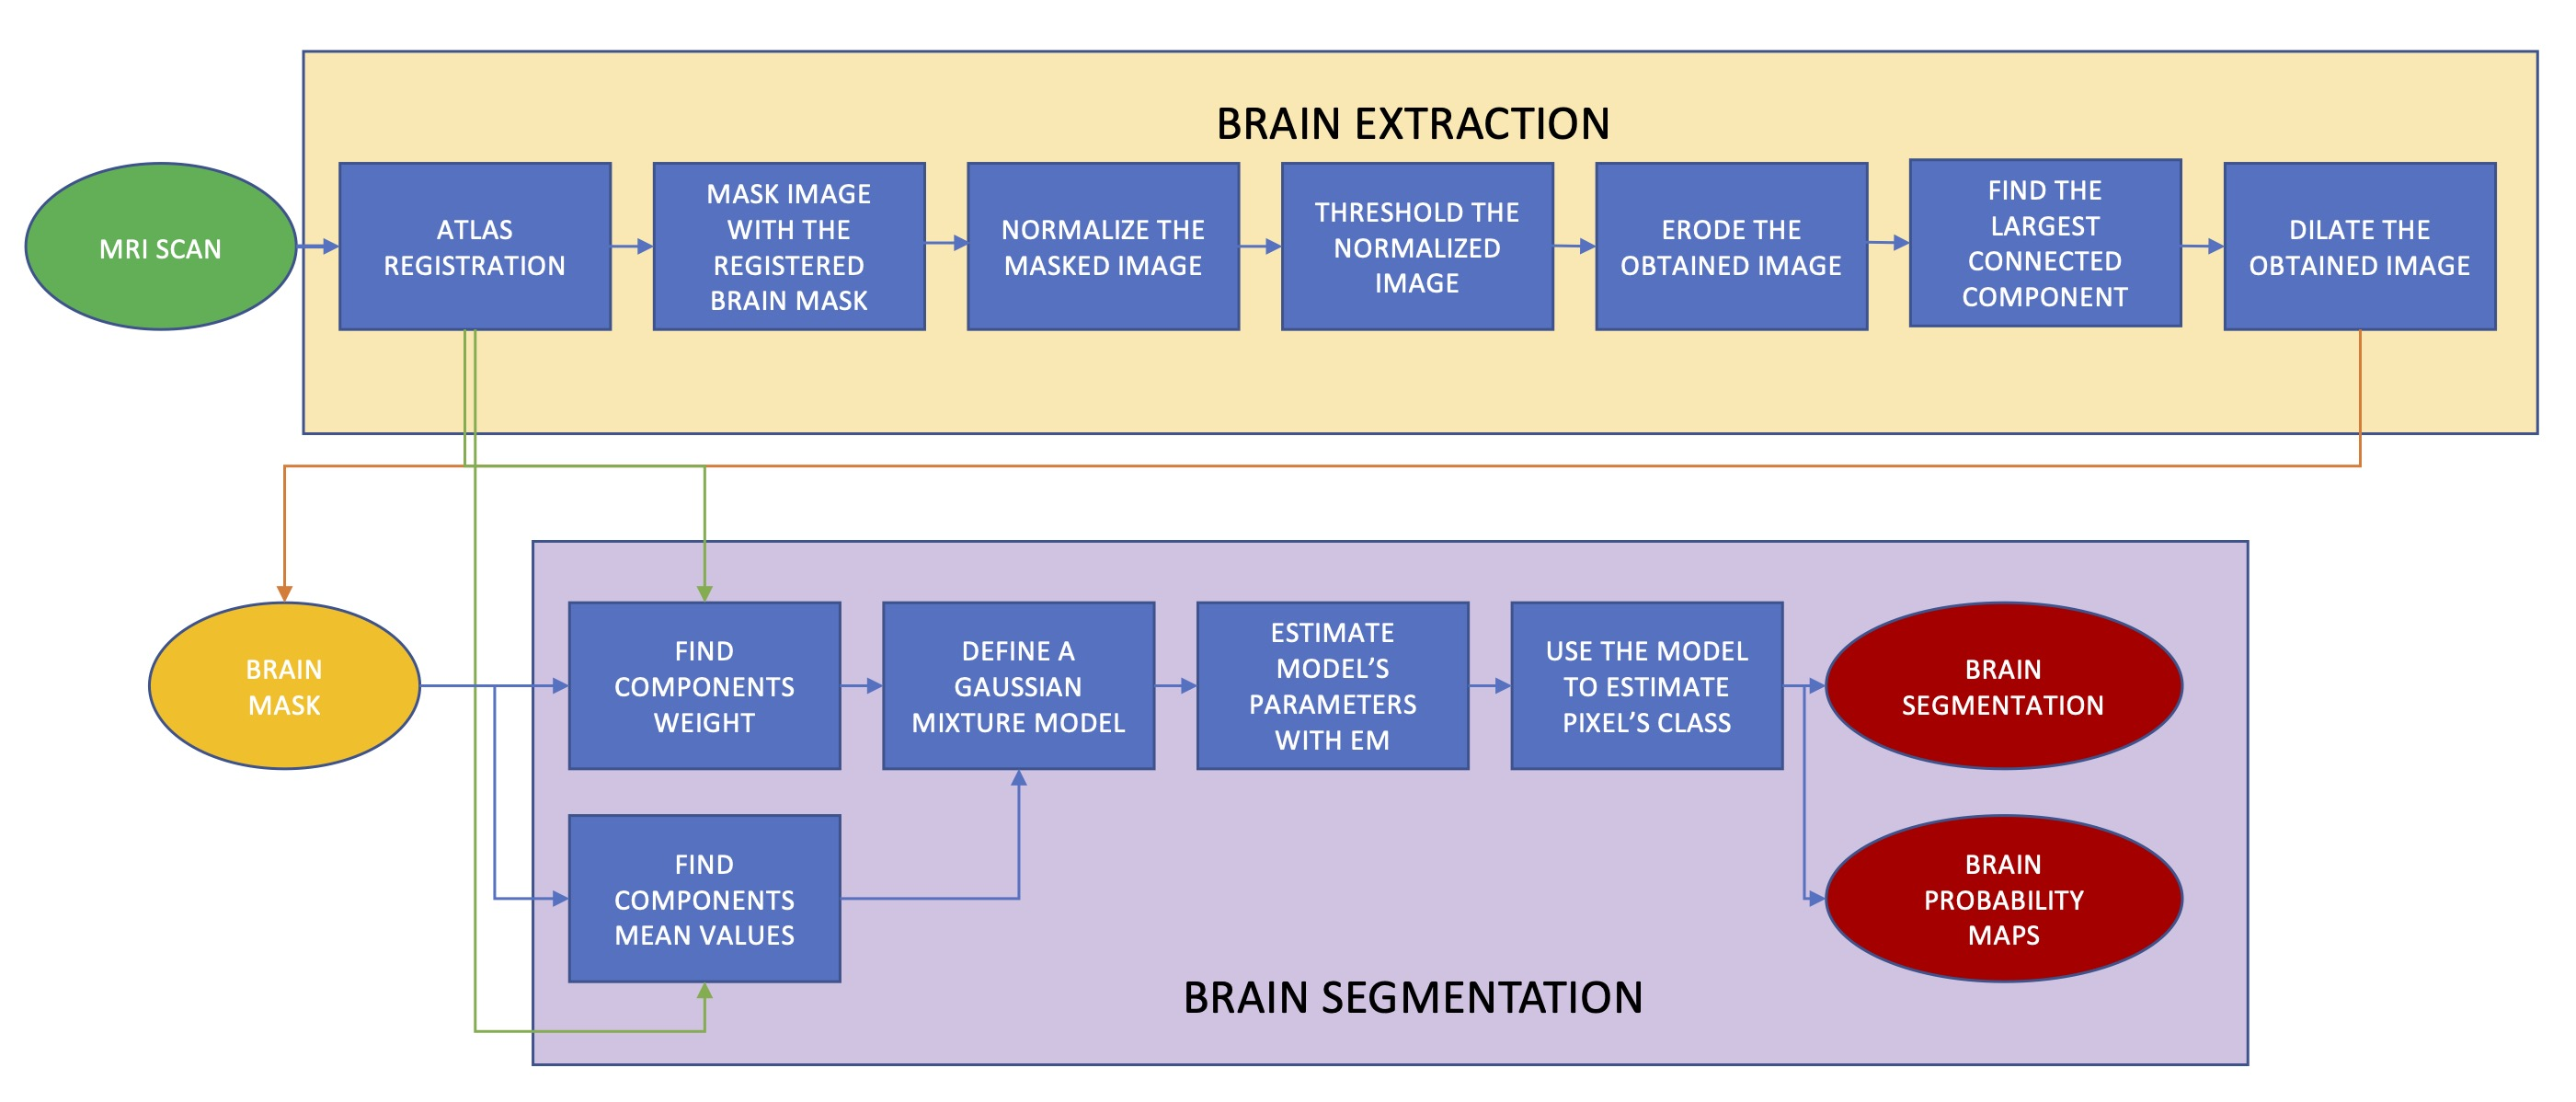
\includegraphics[scale = 0.155]{img/Chap2/FLOWCHART_PRE.jpg}
    \caption{Workflow of the developed preprocessing pipeline. In this flowchart are included both the brain extraction stage and the segmentation stage. The output from the first stage is linked as input of the second stage since only the extracted brain was used during the segmentation process. The atlas registration is linked to the segmentation stage because the probability maps of the atlas was registered in the brain space using the transformation parameters obtained during the registration of the atlas in the brain extraction step.}
    \label{fig:flowchart_pre}
\end{figure}

\subsection{Description}

The first need was to remove from the images everything except the brain, in a step called \textit{brain extraction} (or also \textit{skull stripping}). 
Once this task was done the challenge has been to segment the different brain tissues (white matter, grey matter and cerebrospinal fluid), with special regard toward the white matter, because it is the tissue where SCIs can be found.

The techniques developed for both the brain extraction and the segmentation are atlas based and relies on the use of an already segmented atlas.
The pipeline is designed to work with every atlas that contains at least a brain mask and a soft segmentation of the three tissues cited, but during the developing of this work of thesis was used in particular the ICBM MNI 152 non linear symmetric atlas 2009a which have isotropic voxels of size $1mm^3$  and a total size of $106 \times 232 \times 188$ \cite{MNI152_09a}.




\subsubsection{Brain Extraction}

The process of brain extraction consists in the separation of the brain from the non-brain tissues present in the head. This process is often called also \textit{skull-stripping} even if the two meanings are not totally interchangeable \cite{ART:Han}, it is common to use both the terms to indicate the same process and in this work both the terms will be used. 

This is a common pre-processing step in neuroimaging as it permits to focus only to the spatial volume where the researched features physically are. 
Due to high variability that is possible to find between each image, caused by differences in image acquisition or inter-patient variability the automatic brain extraction is not a easy task.

The technique here proposed is intended to be totally automatic and computationally fast even on a domestic pc. It relies on the use of an atlas and the corresponding binary brain mask.
In that paragraph all the steps that brought to a proper brain extraction are explained.



\paragraph{Registration:}
MNI152 atlas was registered onto the T1W image using a multiodal and multiresolution registration. 
The first transformation used was a \emph{rigid} transformation to roughly align the atlas on the T1 image.
The so obtained image was then transformed with an \emph{affine} transformation to permit to the moving image to scale and skew to reach a better alignment with the fixed image.
In the last step an elastic \emph{BSpline} transformation was applied, to permit the deformation necessary to make the two images as overlapping as possible.
In all those three transformations the metric to minimize was the \emph{mutual information} which allows fast computation of the metric value \cite{Elastix_manual} and permits to match the images even when the  values of the matched pixel are not the same.
Morevoer, according with the last applied transformation, the chosen interpolator was a BSpline function in order to have a higher precision in the final pixel values, since the computation time is not affected in a significant way.
The final result is visible in Figure \ref{fig:atlas_registration}.

\paragraph{Masking:} The mask obtained from the registration was then thresholded and dilated with a spherical kernel of radius $1$. The brain mask obtained was then used to mask the image in order to have a first roughly extracted brain.
The dilating process was necessary in order to obtain a more conservative extraction of the brain and assuring that all the regions of interest were conserved.

\paragraph{Thresholding:}
That allows to reach a rough head segmentation in which only the brain and part of the skull are visible. 
The image obtained in such way was then normalized. The normalization was done calculating the mean value an the standard deviation for the pixels under the mask obtained in the precedent step and then shifting the pixel values in order to have the mean value at 0 and scaling the values of $1 \sigma$.
The normalized image was then thresholded with a multi-otsu algorithm in order to exclude the background and obtain a binary image.
The thresholded image was used as a mask on the original head image.
The obtained masked image was then normalized and thresholded again with a fixed threshold.
Those two thresholds were necessary to have a better control in removing the unwanted regions.
The normalization process was necessary in order to have the possibility of use a fixed threshold.
 
\paragraph{Finding the Largest Connected Region:}
The result from the last step was a binary image in which the gap between the brain and the skull was partially considered background. In order to have a proper separation of the skull from the brain an eroding filter with a spherical kernel of radius $1$ was applied.
At this point, having the brain totally divided from the skull, the largest connected region in the image was found, resulting in the brain.

\paragraph{Refinition:}
The so obtained mask was finally dilated with a spherical kernel of radius $2$, in order to regain the loss volume in the eroding applied for the purpose of fully divide the skull from the brain.


In this way was possible to obtain an algorithm that compute the brain mask for a T1W MRI scan like the ones visible in Figure \ref{fig:skull_stripping} and Figure \ref{fig:skull_stripping_3d} with times in the order of few minutes, even using a normal domestic pc.


\begin{figure}[h!]
		\centering
        \begin{subfigure}[b]{0.325\textwidth}
             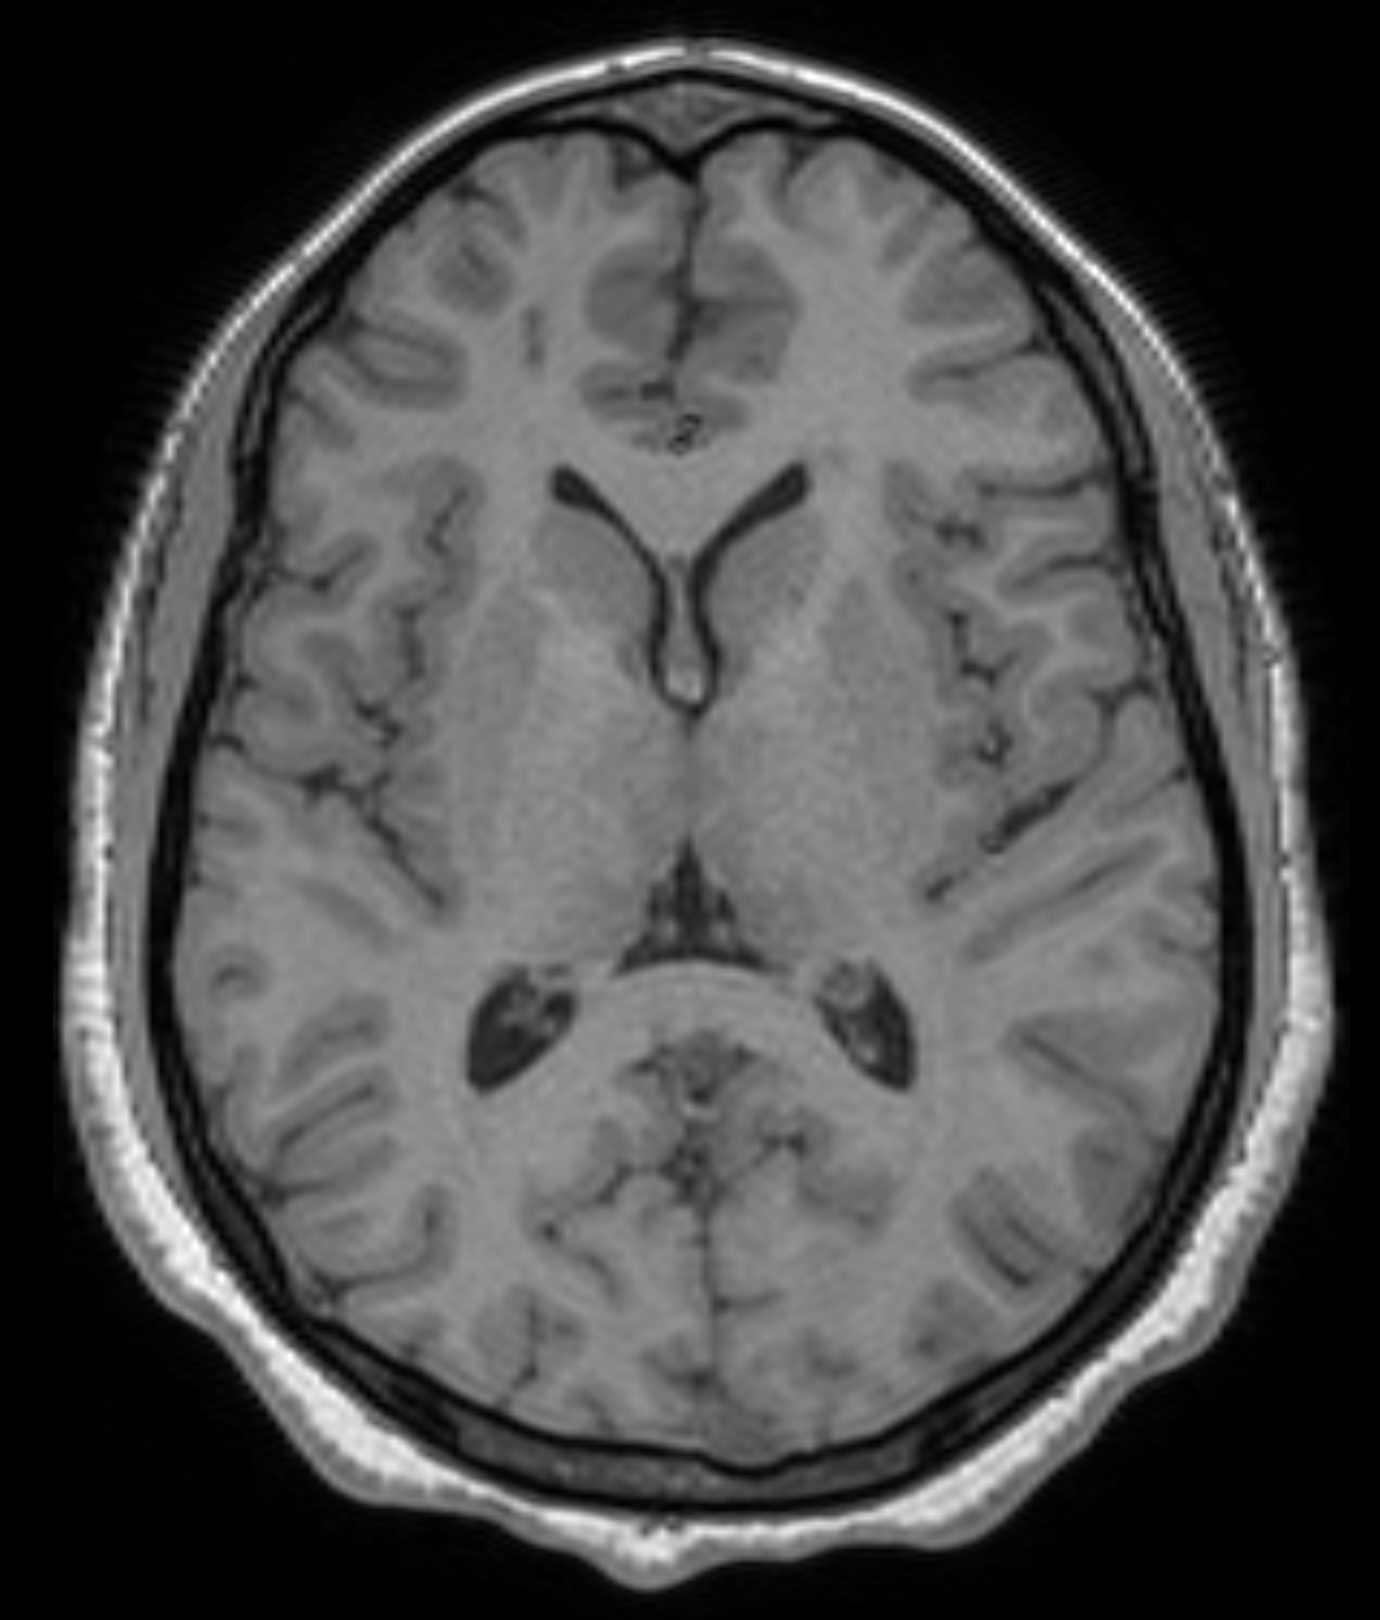
\includegraphics[scale=0.1]{img/Chap2/T1.jpg}
             \caption{Fixed Image}
             \label{fig:T1_atlas}
        \end{subfigure}
        \hfill
        \begin{subfigure}[b]{0.325\textwidth}
             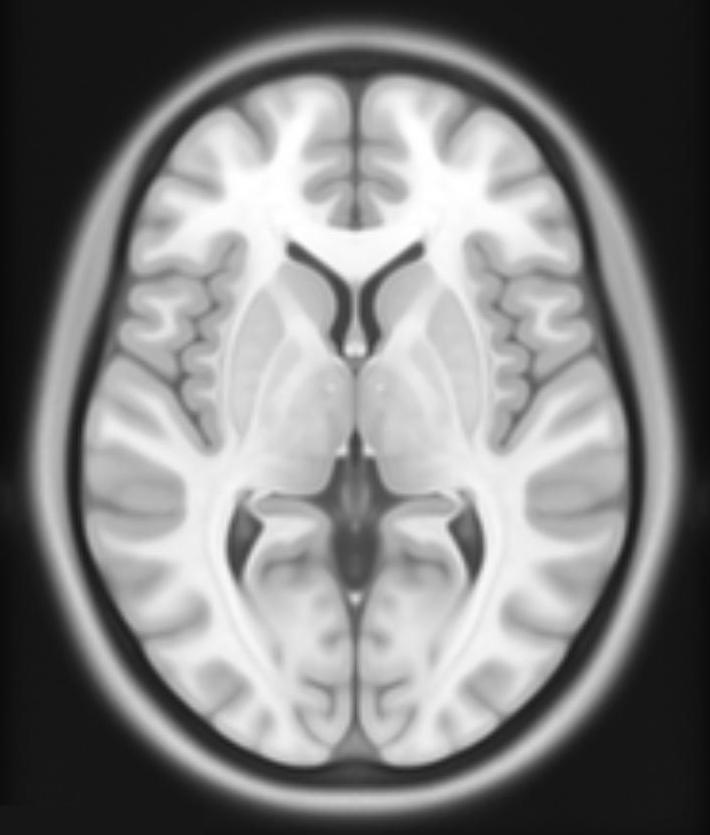
\includegraphics[scale=0.194]{img/Chap2/atlas.jpg}
             \caption{Original Moving Image}
             \label{fig:mni}
        \end{subfigure}
        \hfill
        \begin{subfigure}[b]{0.325\textwidth}
             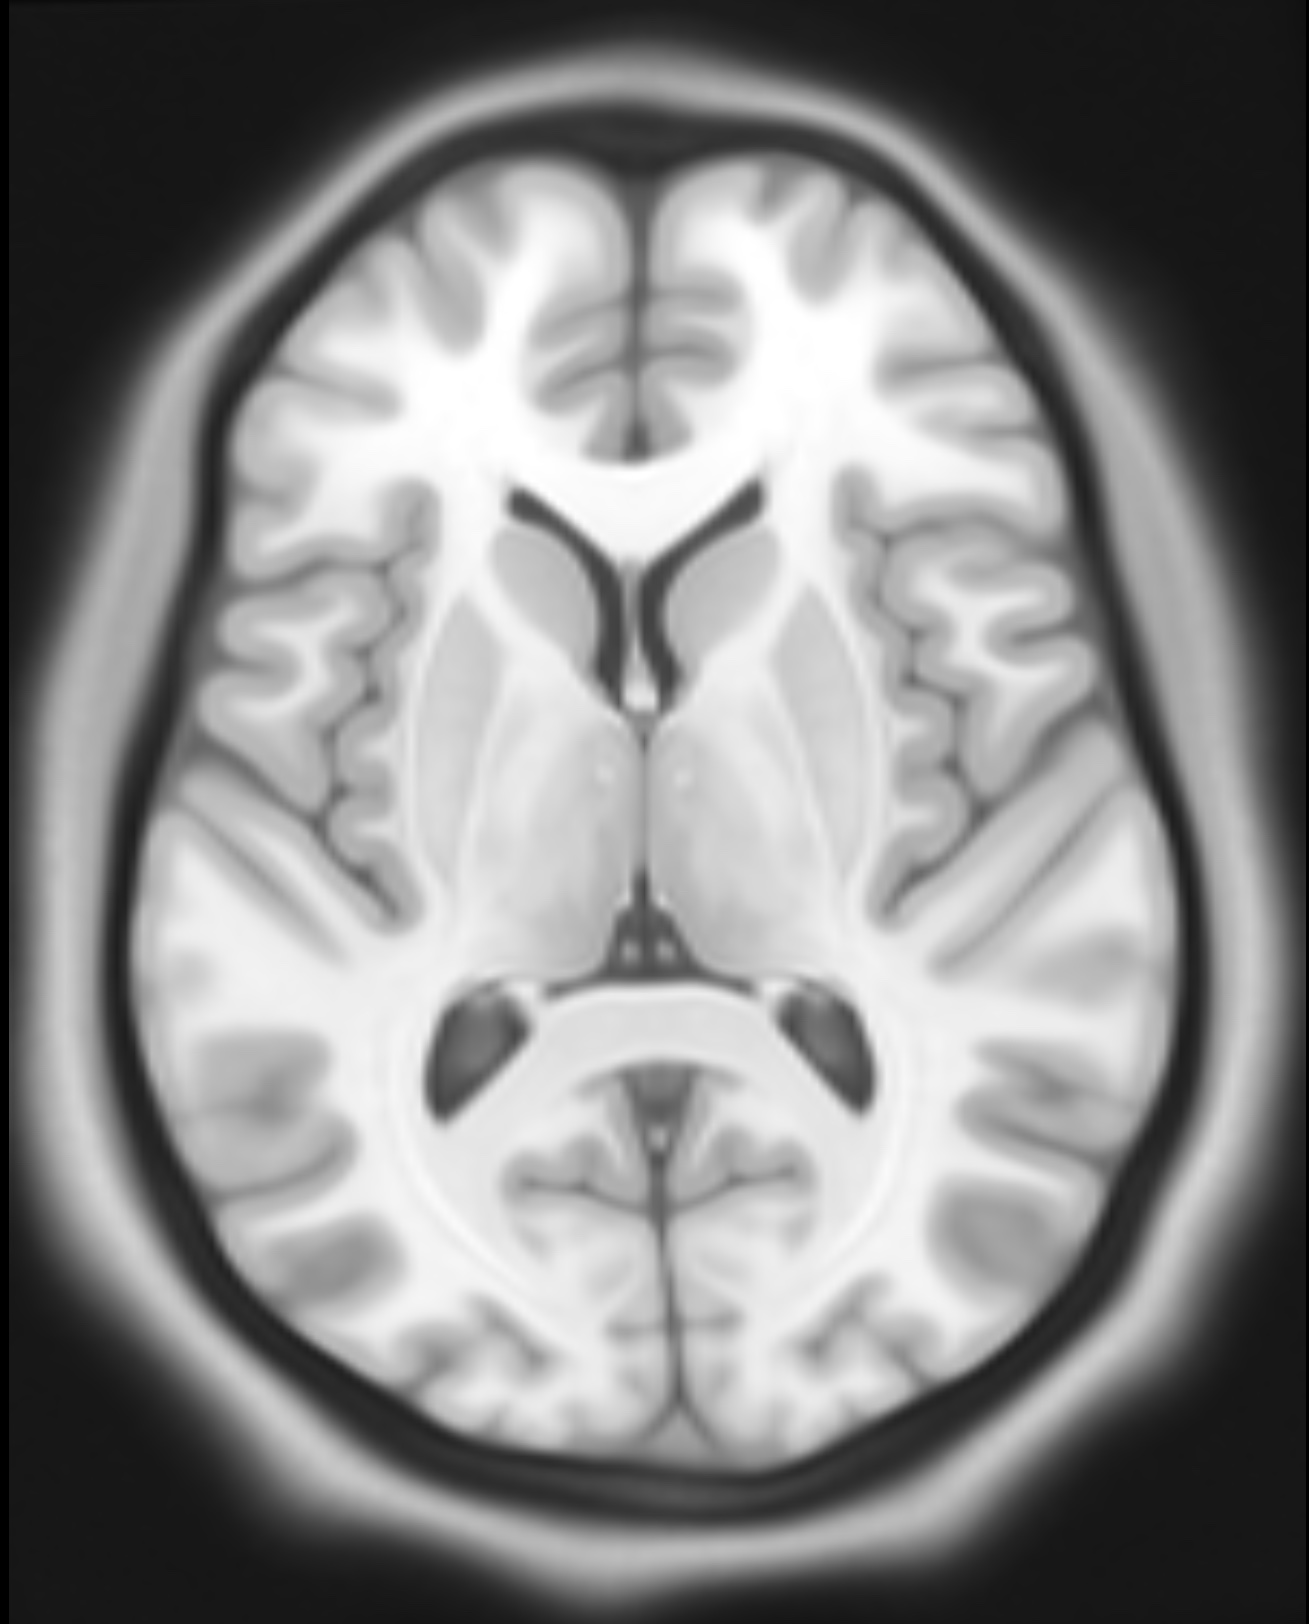
\includegraphics[scale=0.1]{img/Chap2/registered_atlas.jpg}
             \caption{Registered Moving Image}
             \label{fig:registered_mni}
        \end{subfigure}
		\caption{T1W atlas registration over a T1W image. Figure a is the original head scan. Figure b is the MNI 152 \cite{MNI152_09a} atlas before the registration process. Figure c is the atlas scan after the registration and is possible to see how the atlas was deformed by the algorithm to match the fixed image.}
		\label{fig:atlas_registration}
	\end{figure} 


\begin{figure}[h!]
		\centering
        \begin{subfigure}[b]{0.325\textwidth}
             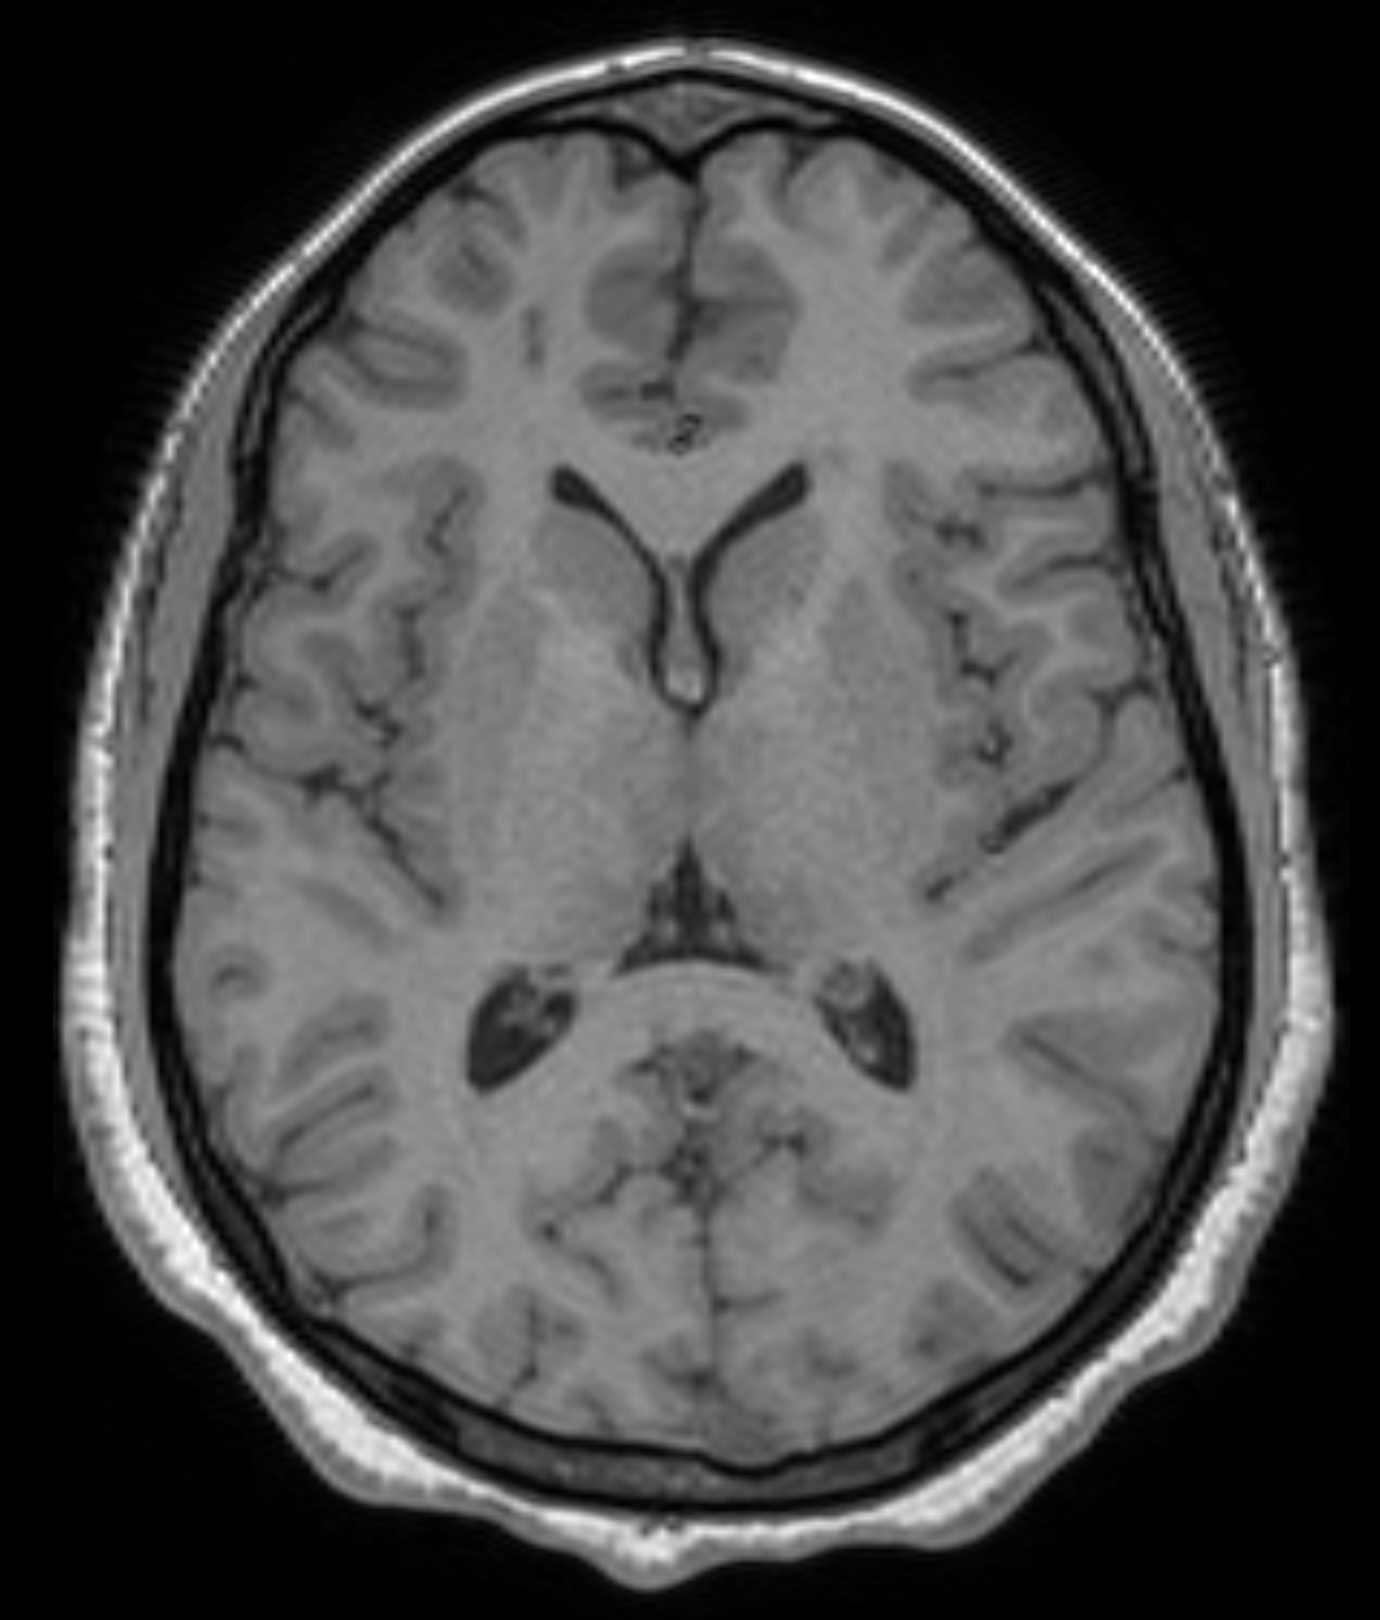
\includegraphics[scale=0.105]{img/Chap2/T1.jpg}
             \caption{Original Image}
             \label{fig:T1_brain}
        \end{subfigure}
        \hfill
        \begin{subfigure}[b]{0.325\textwidth}
             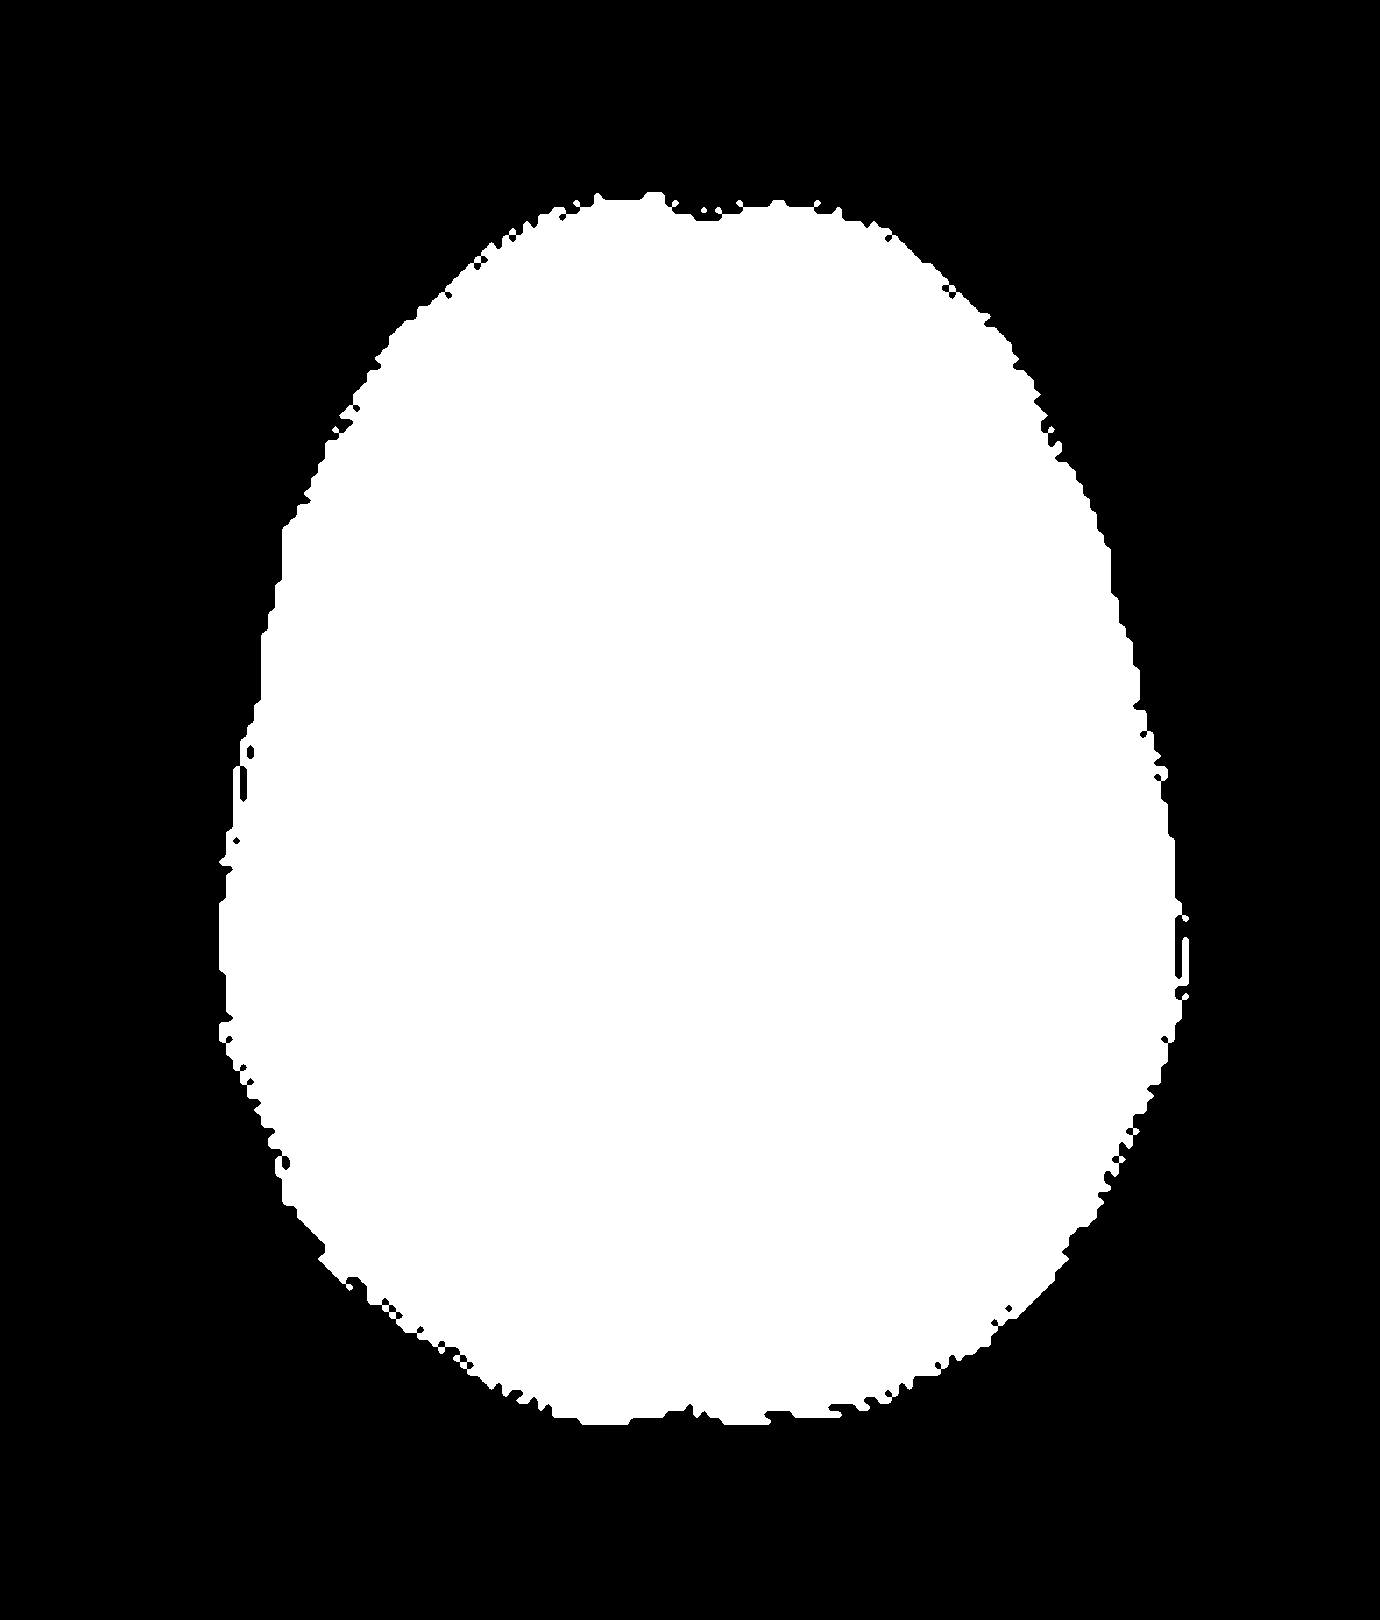
\includegraphics[scale=0.105]{img/Chap2/brain_mask.png}
             \caption{Computed brain mask}
             \label{fig:brain_mask}
        \end{subfigure}
        \hfill
        \begin{subfigure}[b]{0.325\textwidth}
             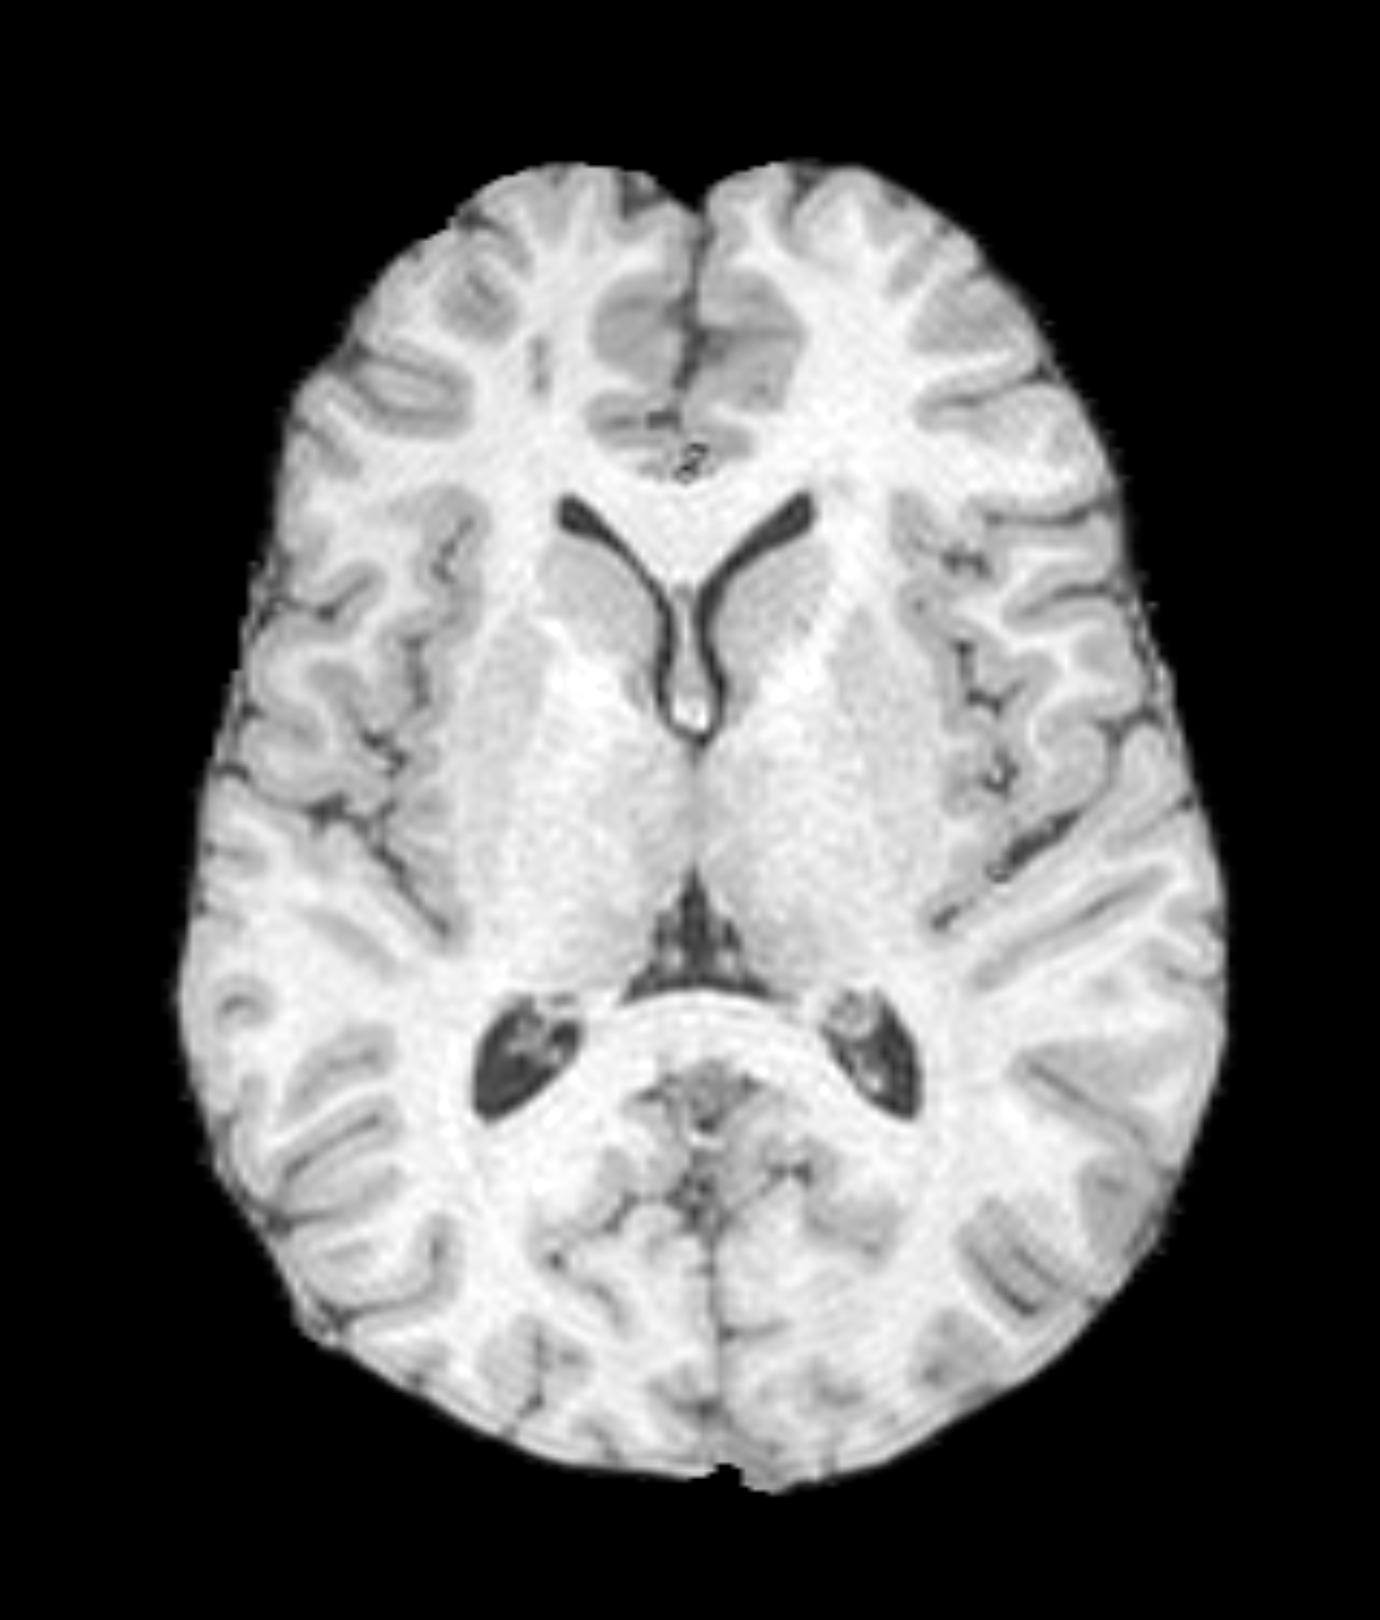
\includegraphics[scale=0.105]{img/Chap2/brain.jpg}
             \caption{Extracted brain}
             \label{fig:brain}
        \end{subfigure}
		\caption{In these images is possible to see the comparison between an original head image (a), the brain mask computed (b) and the brain extracted with that mask (c). }
		\label{fig:skull_stripping}
	\end{figure} 
	

\begin{figure}[h!]
    \centering
             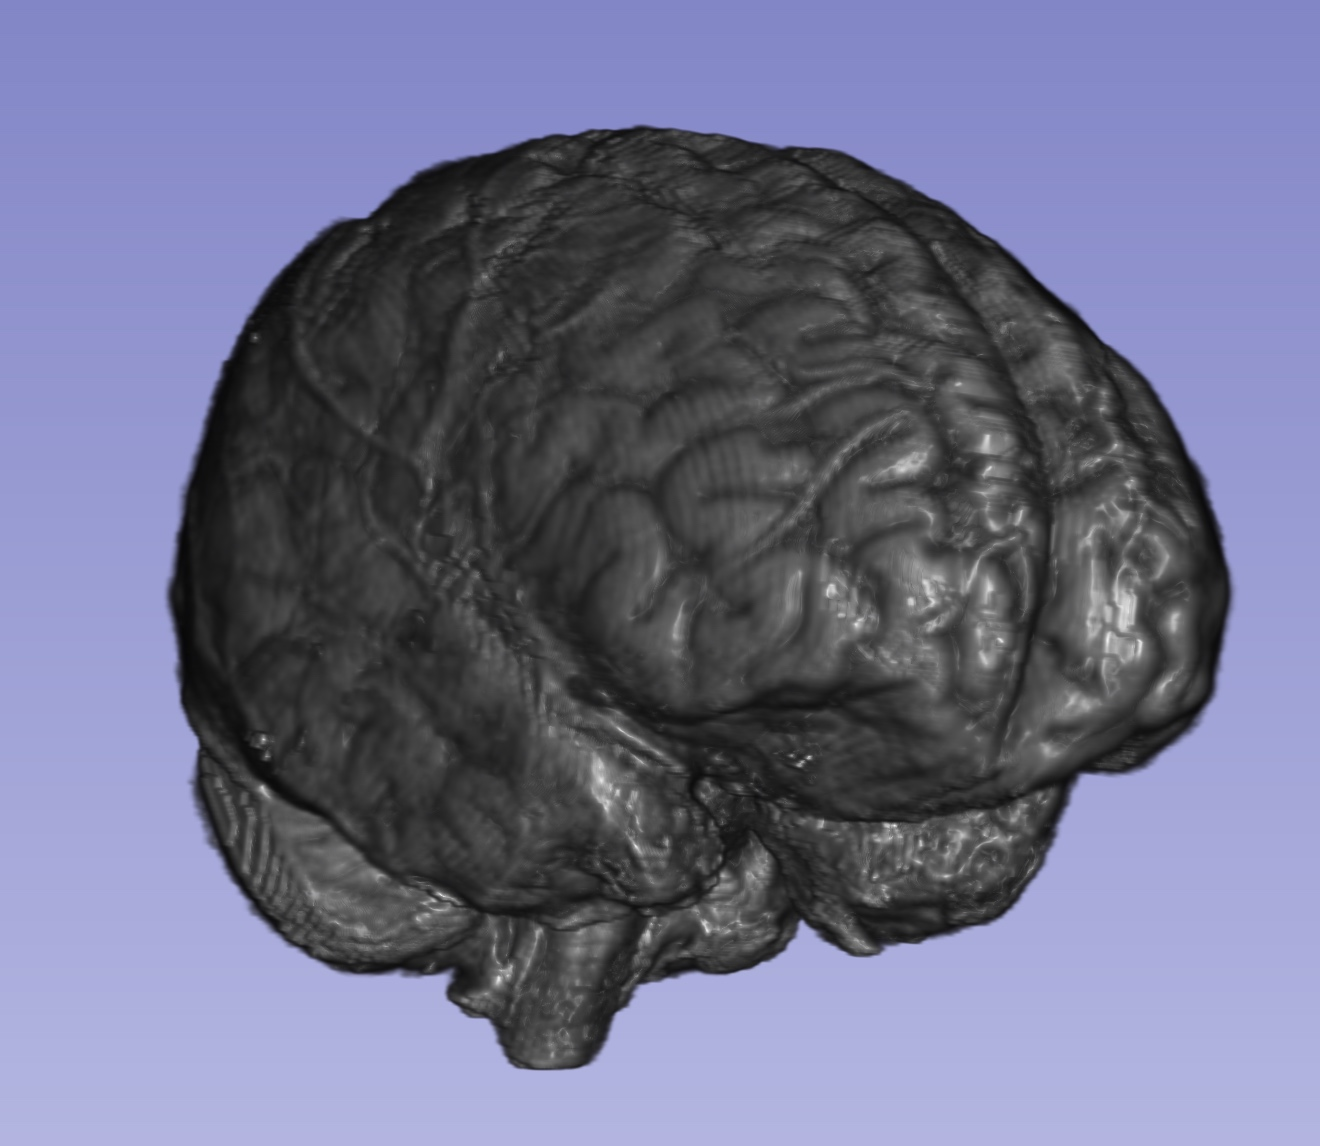
\includegraphics[scale=0.32]{img/Chap2/3Dbrain.jpg}
		\caption{Using specialized applications is possible to render a 3D image of the volumes permitting to have a better looking to the external structures of the obtained object. The one here proposed let see the extracted brain with the proposed algorithm. The image is the same of Figure \ref{fig:skull_stripping}. This 3D rendering is computed with the application 3DSlicer \cite{3DSlicer}.}
		\label{fig:skull_stripping_3d}
	\end{figure} 





\subsubsection{Tissue Segmentation}

Since the SCIs are found only in the white matter, a proper segmentation of the brain tissues has a great value for their segmentation. 
For the aims of this work of thesis the algorithm is intended to work with relatively short time even on a normal domestic personal computer.

The main idea behind the approach here proposed was to consider the pixel values of the brain distributed as a mixture of Gaussians distributions, as visible in Figure\ref{fig:brain_histogram} and then use an Expectation Maximization (EM) algorithm to estimate the parameters for those distribution functions. 
The EM algorithm requires some parameters for it initialization, such as the number of classes, the estimated mean value for each class and the weight of each class on the total image.
The potentiality of having the brain already extracted was to have the background already segmented and therefore the number of classes was set to $3$ as the algorithm is intended to segment the main tissues of the brain (white matter, grey matter, cerebrospinal fluid).
The other parameters were estimated relying on the registration of the probability maps for the tissue segmentation of the atlas on the images.
This approach permits an initialization more accurate and focused for each analysed volume.

In the first place the probabilistic tissue maps of the atlas were transformed using the same transformation obtained for the atlas registration during the skull stripping.
Once the map were transformed each pixel was assigned to the class with the higher probability.
This process permitted to have a rough preliminary segmentation of the tissues and this information was used to compute the estimate for the class weight and the mean value of the pixels of every tissue.

It is to mention that the expectation maximization algorithm lead to a soft segmentation, giving a probability map for every class in output. To compute the hard segmentation was used the same approach as before: every pixel was assigned to the class of greater probability.
The results of the segmentation are visible in Figure\ref{fig:postprocessing}.

\begin{figure}
    \centering
    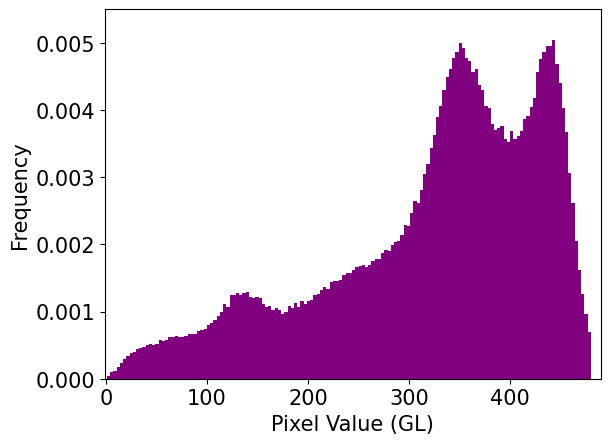
\includegraphics[scale = 0.95]{img/Chap2/histogram.png}
    \caption{In the figure is possible to see the histogram of an extracted brain from a T1W scan. Looking at the pixel value distribution (expressed as Grey Level since it is a monochromatic image) is possible to appreciate how to model the pixel distribution as a mixture of Gaussians with different means (identifiable with the three observable peaks) and different standard deviations.}
    \label{fig:brain_histogram}
\end{figure}

\begin{figure}[h!]
		\centering
        \begin{subfigure}[b]{0.495\textwidth}
             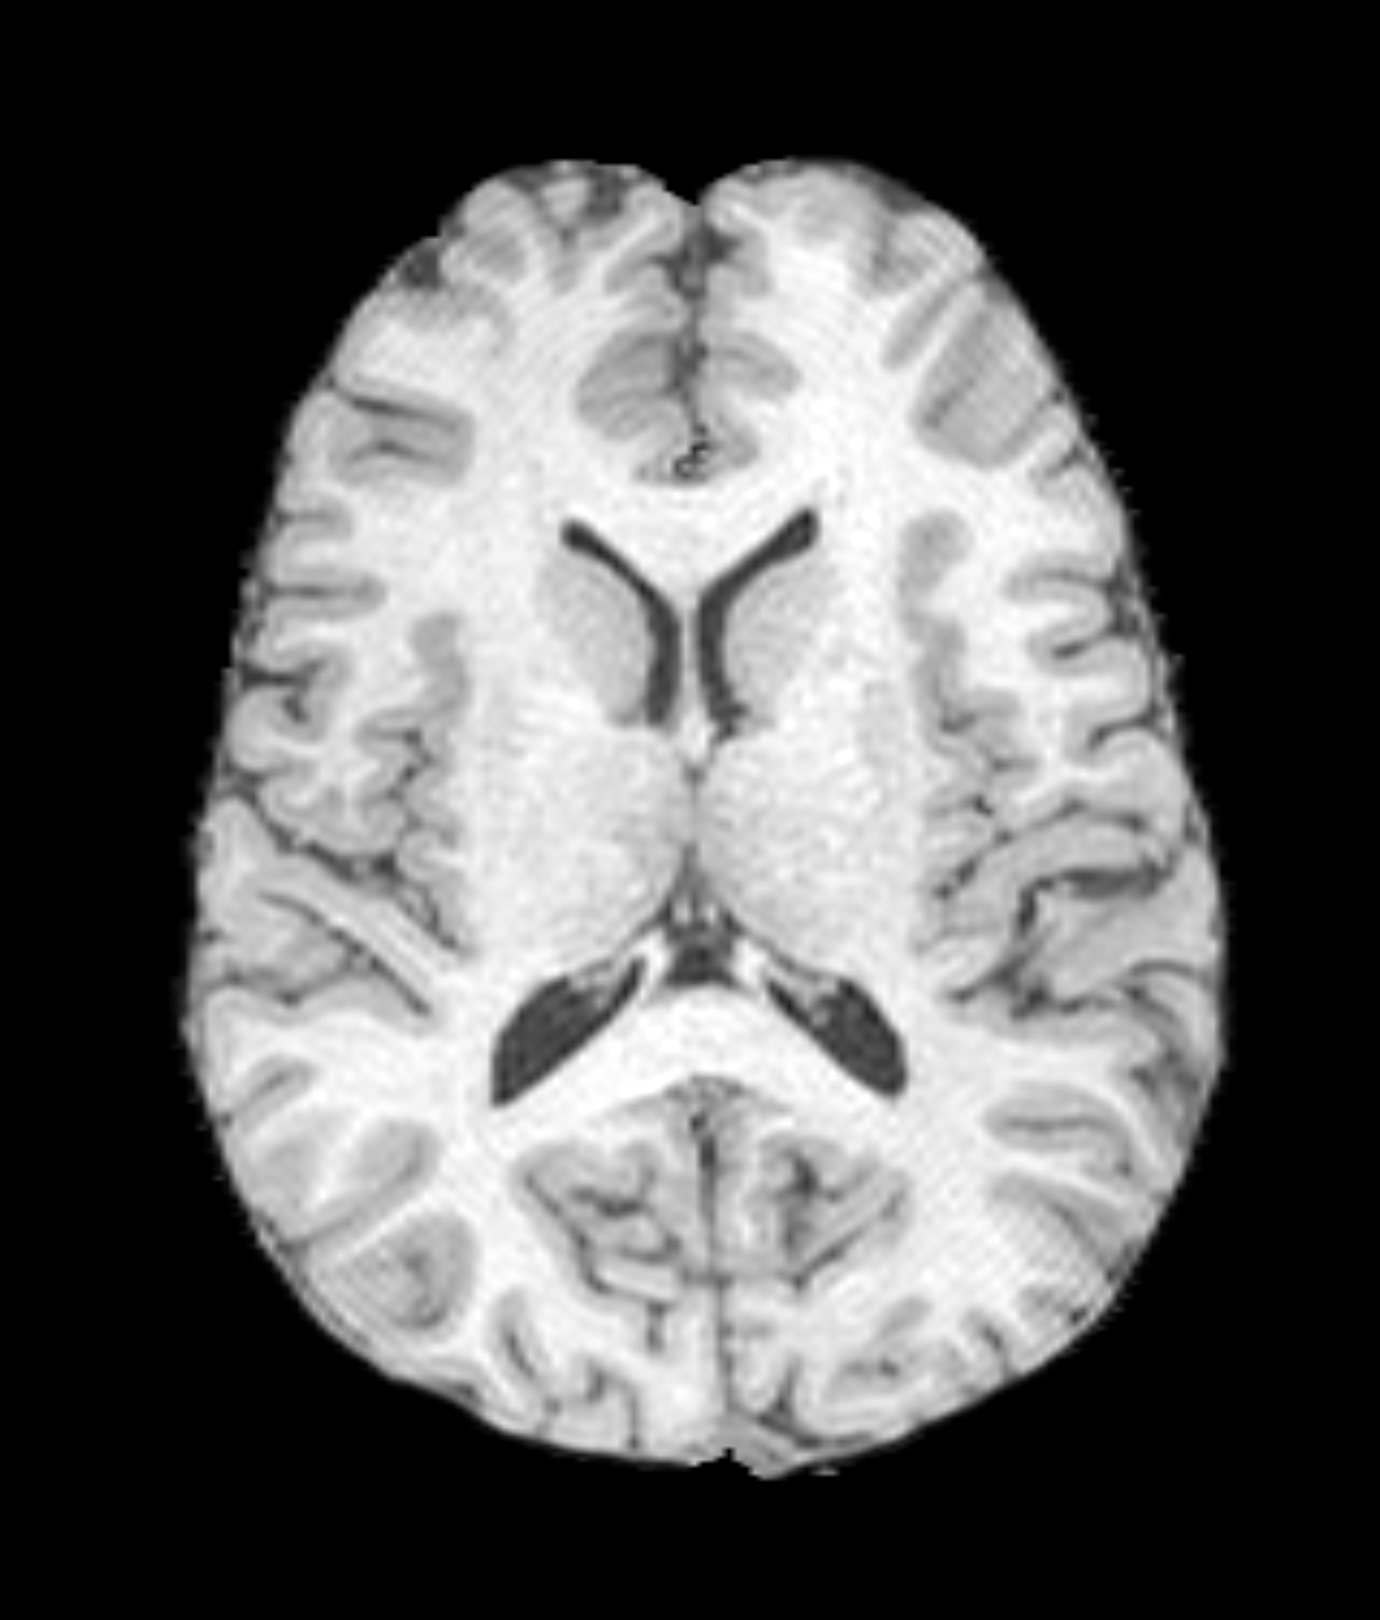
\includegraphics[scale=0.15]{img/Chap2/brain2.jpg}
             \caption{Brain extracted from a T1W scan.}
        \end{subfigure}
        \hfill
        \begin{subfigure}[b]{0.495\textwidth}
             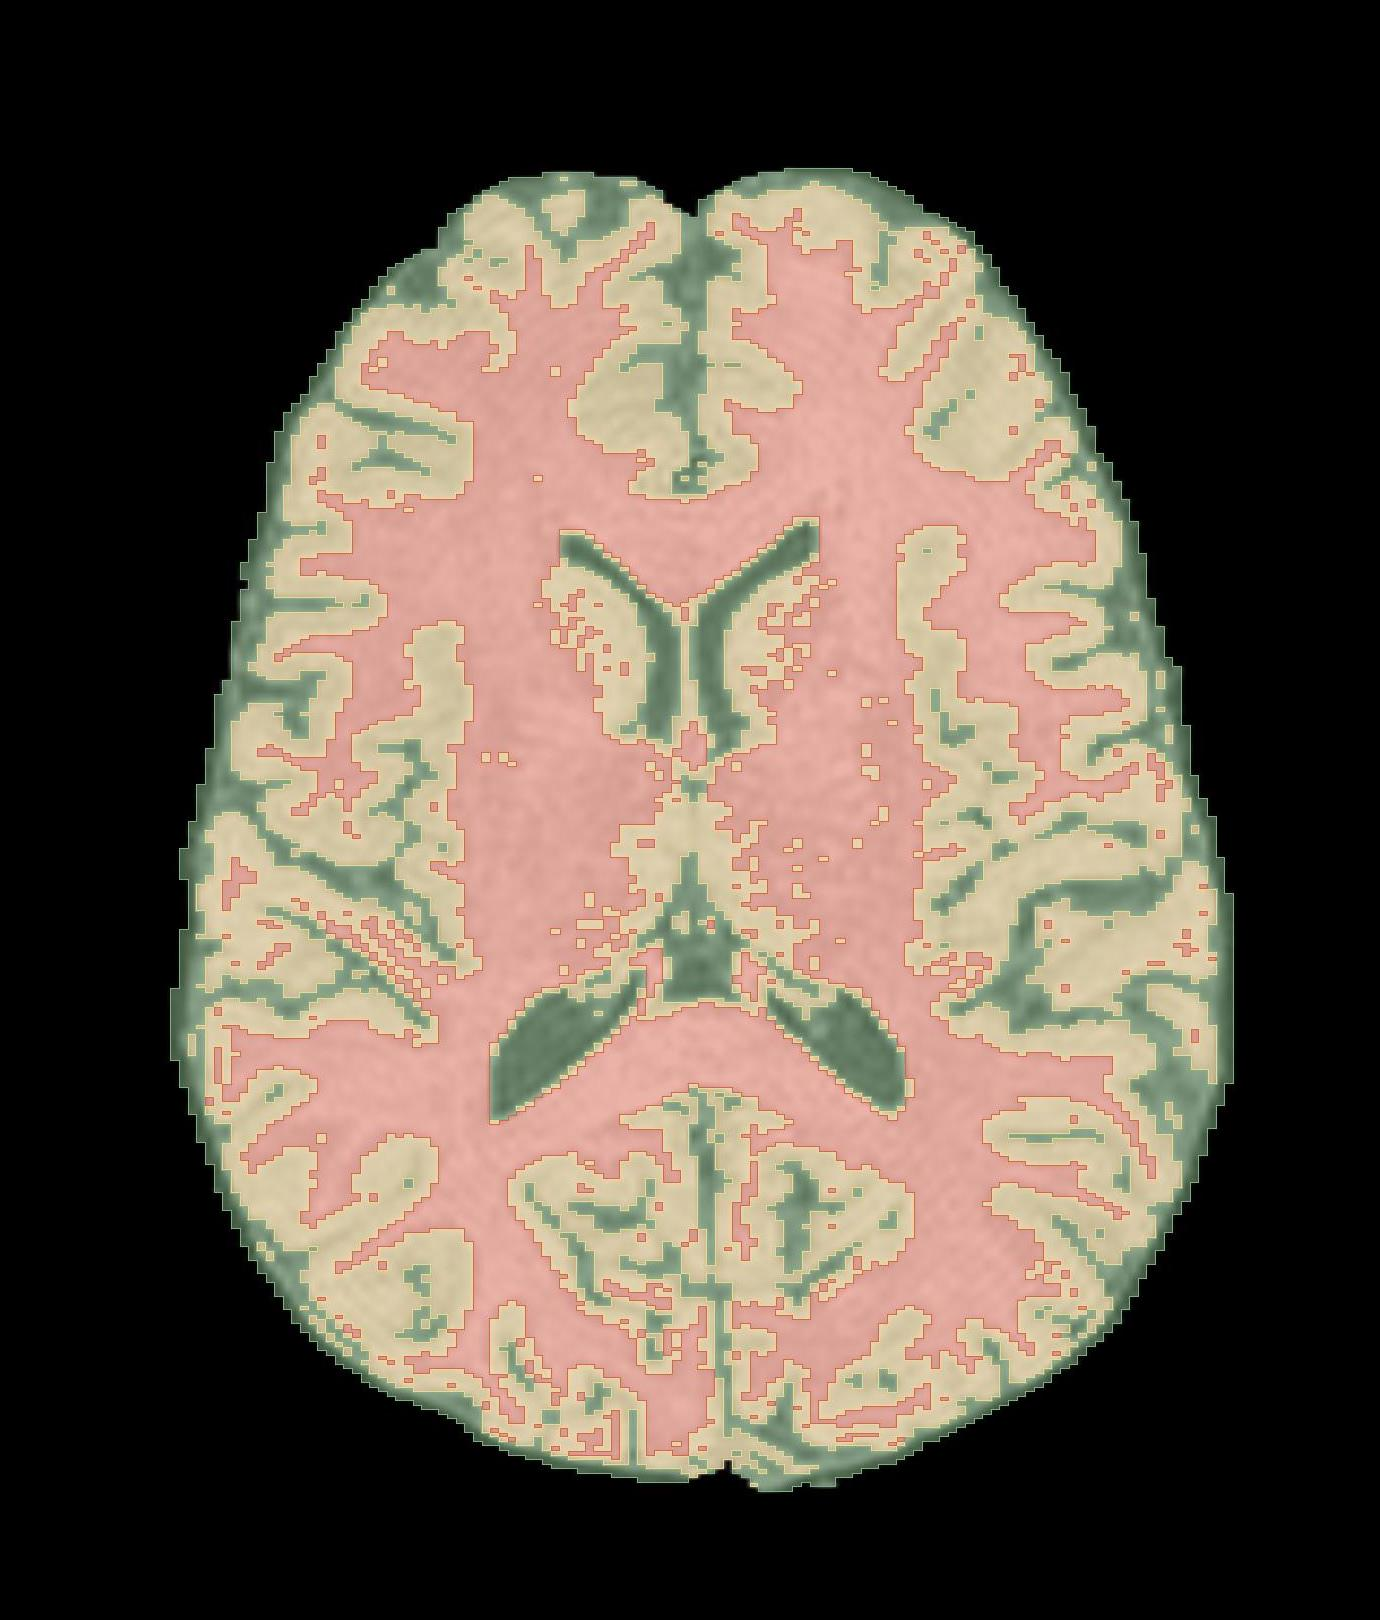
\includegraphics[scale=0.15]{img/Chap2/segmented_axial.jpg}
             \caption{Brain segmentation result.}
        \end{subfigure}
        \caption{Segmentation process results on an already extracted brain. Figure a is the brain extracted from the scan. In Figure b is is possible to observe the result of the segmentation process in which the white matter is labeled in red, the grey matter in yellow and the cerebrospinal fluid in green.
        The masks are obtained from a Gaussian mixture model with three classes which parameters were estimated using an expectation maximization algorithm.}\label{fig:postprocessing}
\end{figure}

\subsection{Implementation}

The two pipelines described before was implemented using Python, which is an high level object oriented programming language. To perform all the essential operations (input/output, filtering, morphological operations, etc.) two main libraries were used: \textsc{ITK} \cite{ART:ITK} and \textsc{Numpy} \cite{Numpy}. To perform the registration and to apply the obtained transformations the \textsc{ITK-Elastix} \cite{ITK-Elastix} library was used, which is an ITK Python interface to Elastix \cite{ART:Elastix}. To implement the brain segmentation the \textsc{Scikit-Learn}\cite{scikit-learn} library was used. 

The whole code is opensource and freely available con GitHub \cite{Neuroradiomics} and the installation is managed by a setup.py file which also provides the full list of dependencies.
During the developement, the installation was automatically tested on Ubuntu for different python versions. This continuos integration process was carried out using the github actions.

The whole code is subdivided in three modules, respectively dedicated to registration, skull stripping and segmentation and is intended to work with Nifti images.

\subsubsection{Brain Extraction}

In the last years many methods were proposed. Some of the more widely used examples of brain extraction methods are \emph{Brain Extraction Tool (BET)} from the FSL library, \emph{Brain Surface Extraction (BSE)} which is part of BrainSuite and \emph{Robust Learning-based Brain Extraction System (ROBEX)} and many others \cite{ART:Han}.
Each of the cited methods have a different approach to the skull stripping problem, ranging from low level morphological operations to the classification using pattern recognition.

The brain extraction process proposed in this work of thesis relies on a registration of an atlas over the image as explained before, so both the registration module and the skull stripping module are involved in this part of the implementation.

The registration was done using this function based on Elastix library.
The images were all read with the ITK I/O functions with floating pixels as required by Elastix.

\documentclass{standalone}




\begin{document}




\lstset{style=python}
	\begin{lstlisting}[language=python, caption=Multimap Registration Function, label=multimap_registration]
import itk
	
def elastix_multimap_registration(fixed_image, moving_image):
    
    # Setting our number of resolutions
    parameter_object = itk.ParameterObject.New()
    resolutions = 4
    
    #Import RIGID parameter map
    parameter_map_rigid = parameter_object.GetDefaultParameterMap(
    'rigid', resolutions)
    parameter_map_rigid['Metric']       = [                                    'AdvancedMattesMutualInformation']
    parameter_map_rigid['Interpolator'] = [
    'BSplineInterpolatorFloat']
    parameter_object.AddParameterMap(parameter_map_rigid)
    
    #Adding an AFFINE parameter map
    parameter_map_affine = parameter_object.GetDefaultParameterMap(
    "affine", resolutions)
    parameter_map_affine['Metric']       = [
    'AdvancedMattesMutualInformation']
    parameter_map_affine['Interpolator'] = [
    'BSplineInterpolatorFloat']
    parameter_object.AddParameterMap(parameter_map_affine)
    
    #Adding a NON-RIGID parameter map
    parameter_map_bspline = parameter_object.GetDefaultParameterMap(
    "bspline", resolutions)
    parameter_map_bspline['Interpolator'] = [
    'BSplineInterpolatorFloat']
    
    parameter_object.AddParameterMap(parameter_map_bspline)
    
    #Set the registration
    elastix_object = itk.ElastixRegistrationMethod.New(
                                            fixed_image, moving_image)
    elastix_object.SetParameterObject(parameter_object)
    
    #Start the registration
    elastix_object.UpdateLargestPossibleRegion()
    
    return elastix_object
\end{lstlisting}


\end{document}

At the end of the registration and object containing both the registered image and the transformation applied was returned. This function is then inserted in the the main brain extraction pipeline. 

The implemented pipeline use different functions that are aimed to perform the different steps described in the previous sections.
The first needs encountered was to have a simple interface for the application of the used ITK filters, as threshold and morphological operations and their name is always self explanatory.

% \documentclass{standalone}




\begin{document}




\lstset{style=python}
	\begin{lstlisting}[language = python, caption = Wrapped ITK filters, label =multimap_registration]
import itk
	
def binarize ( image, low_value = 0.1, hi_value = None ):
    
    thresholdFilter = itk.BinaryThresholdImageFilter[OutputType, OutputType].New()
    thresholdFilter.SetInput(c_image)
    thresholdFilter.SetLowerThreshold(low_value)
    thresholdFilter.SetOutsideValue(0)
    thresholdFilter.SetInsideValue(1)
        
    if hi_value != None : 
        thresholdFilter.SetUpperThreshold(hi_value)

    thresholdFilter.Update()
    
    return thresholdFilter.GetOutput() 
	

def normal_threshold ( image, value ):
    
    thresholdFilter = itk.BinaryThresholdImageFilter[type(image), type(image)].New()
    thresholdFilter.SetInput(image)
    thresholdFilter.SetLowerThreshold(-value)
    thresholdFilter.SetUpperThreshold(value)
    thresholdFilter.SetOutsideValue(0)
    thresholdFilter.SetInsideValue(1)
    thresholdFilter.Update()

    return thresholdFilter.GetOutput()


def binary_eroding (image, radius = 1):
    
    struct_element = itk.FlatStructuringElement[3].Ball(radius)
    
    erodingFilter = itk.BinaryErodeImageFilter[type(image), type(image), type(struct_element)].New()
    erodingFilter.SetInput(image)
    erodingFilter.SetKernel(struct_element)
    erodingFilter.SetBackgroundValue(0)
    erodingFilter.SetForegroundValue(1)
    erodingFilter.Update()
    
    return erodingFilter.GetOutput()

    
def binary_dilating (image, radius=1):

    struct_element = itk.FlatStructuringElement[3].Ball(radius)

    dilatingFilter = itk.BinaryDilateImageFilter[type(image), type(image), type(struct_element)].New()
    dilatingFilter.SetInput(image)
    dilatingFilter.SetKernel(struct_element)
    dilatingFilter.SetDilateValue(1) 
    dilatingFilter.Update()
    
    return dilatingFilter.GetOutput()


def hole_filler(image):
    
    hole_filler_filter = itk.BinaryFillholeImageFilter[OutputType].New()
    hole_filler_filter.SetInput(cast_filter.GetOutput())
    hole_filler_filter.SetForegroundValue(1)
    hole_filler_filter.Update()
    
    return hole_filler_filter.GetOutput()

\end{lstlisting}


\end{document}

One of the most important step in this brain extraction pipeline is the rough masking done with the registered atlas' brain mask. Due to the ITK installation on python, in which not every filter are wrapped from the original C++ language, the masking functions was not always available for the used types. To bypass the problem a dedicated function that explicitly set a $0$ value for every pixel outside the mask was implemented with the name of \emph{negative\_3d\_masking}.

% \documentclass{standalone}

\begin{document}




\lstset{style=python}
	\begin{lstlisting}[language=python, caption = Masking Function, label=negative_masking]
import itk

def negative_3d_masking (image, mask):
    
    Dimension = 3
    ImageType = itk.template(image)[1]
    masked_image = itk.Image[ImageType].New()
    
    masked_image.SetRegions( image.GetLargestPossibleRegion() )
    masked_image.SetSpacing( image.GetSpacing() )
    masked_image.SetOrigin( image.GetOrigin() )
    masked_image.SetDirection( image.GetDirection() )
    masked_image.Allocate()
    
    index = itk.Index[Dimension]()
    
    for index[0] in range( mask.GetLargestPossibleRegion().GetSize()[0] ):
        for index[1] in range( mask.GetLargestPossibleRegion().GetSize()[1] ):
            for index[2] in range( mask.GetLargestPossibleRegion().GetSize()[2] ):
                if mask.GetPixel(index) < 1e-01:
                    masked_image.SetPixel(index, 0)
                else: 
                    masked_image.SetPixel(index, image.GetPixel(index))
    
    return masked_image


\end{lstlisting}

\end{document}

One of the important processes needed to explain in this section is the normalization used to permit the using of a fixed threshold. It permits the normalization of the pixels values masked by a certain mask which in this case is the brain mask obtained in the first steps, permitting to not have the background pixel's value to account for the normalization process.

% \documentclass{standalone}

\begin{document}




\lstset{style=python}
	\begin{lstlisting}[language=python, caption = Normalization functions, label=normalization]
import itk
import numpy as np

def itk_label_shape_statistics( image, labelmap ):

    filter_ = itk.LabelStatisticsImageFilter[ type(image), type(labelmap) ].New()
    _ = filter_.SetLabelInput( labelmap )
    _ = filter_.SetInput( image )

    return filter_


def itk_shift_scale( image, shift = 0., scale = 1. ):

    filter_ = itk.ShiftScaleImageFilter[type(image), type(image)].New()
    _ = filter_.SetInput( image )
    _ = filter_.SetScale( scale )
    _ = filter_.SetShift( shift )

    return filter_


def itk_gaussian_normalization( image, mask, label = 1 ):

    stats = itk_label_shape_statistics( image, mask )
    _ = stats.Update()
    shift = -stats.GetMean( label )
    scale = 1. / abs( stats.GetSigma( label ) )
    normalized = itk_shift_scale( image, shift = shift, scale = scale )

    return normalized


\end{lstlisting}

\end{document}

The last step in the brain extraction is the function that permits to find the largest connected region in the image. This is the step in which the proper brain is extracted.
The function implemented simply found every connected region in the image and then sort them by their dimension, finally keeping only the greater ones.


\documentclass{standalone}

\begin{document}




\lstset{style=python}
	\begin{lstlisting}[language=python, caption = Largest Connected Region Finder, label=find_largest_region]
import itk	
	
def find_largest_connected_region (image):

    #searching for connected regions in the images
    connected_filter = itk.ConnectedComponentImageFilter[OutputType, OutputType].New()
    connected_filter.SetInput(cast_filter.GetOutput())
    connected_filter.Update()
    
    #relabeling the images in increasing order for decreasing dimension
    label_filter = itk.RelabelComponentImageFilter[OutputType, OutputType].New()
    label_filter.SetInput(connected_filter.GetOutput())
    label_filter.Update()
    
    #tengo solo la regione connessa più grande
    thresholdFilter = itk.ThresholdImageFilter[OutputType].New()
    thresholdFilter.SetInput(label_filter.GetOutput())
    thresholdFilter.ThresholdOutside (1,1)
    thresholdFilter.SetOutsideValue(0)
    thresholdFilter.Update()
    
    return thresholdFilter.GetOutput()

\end{lstlisting}

\end{document}


The pipeline for the brain extraction is then implemented as follows.

\documentclass{standalone}




\begin{document}




\lstset{style=python}
	\begin{lstlisting}[language=python, caption=Brain Extraction Function, label=skull_stripping]
	import itk
	import numpy as np
	
	def skull_stripping_mask (image, atlas, mask, transformation_return = False):
	
    reg_atlas_obj = elastix_multimap_registration( image, atlas )
    
    #apply the transformation to the mask and then make it again a binary image
    reg_mask = itk.transformix_filter( mask, reg_atlas_obj.GetTransformParameterObject() )
    bin_reg_mask = binarize( reg_mask )
    
    #dilating the mask to be more conservative
    bin_reg_mask = binary_dilating(bin_reg_mask)
    
    #do a first skull stripping
    first_brain = negative_3d_masking( image, bin_reg_mask )
    
    #binarize the first_brain to obtain a mask useful for the normalization
    first_brain_mask = binarize( first_brain )
    
    #Casting the first_brain_mask to be used by the normalization filter
    OutputType = itk.Image[itk.UC, 3]
    cast_filter = itk.CastImageFilter[type(first_brain_mask), OutputType].New()
    cast_filter.SetInput(first_brain_mask)
    cast_filter.Update()
    first_brain_mask = cast_filter.GetOutput()
    
    #normalize the first obtained brain
    normalized_first_brain = itk_gaussian_normalization( first_brain, first_brain_mask )
    normalized_first_brain.Update()
    
    #Normalized image must be casted
    OutputType = itk.Image[itk.D, 3]
    cast_filter = itk.CastImageFilter[type(normalized_first_brain.GetOutput() ), OutputType].New()
    cast_filter.SetInput(normalized_first_brain)
    normalized_first_brain = cast_filter.GetOutput()
    
    #MultiOtsu thresholding the normalized_brain
    InputType = type(normalized_first_brain)
    motsu = itk.OtsuMultipleThresholdsImageFilter[InputType, InputType].New()
    motsu.SetInput(normalized_first_brain)
    motsu.SetNumberOfThresholds(3)
    motsu.Update()
    thresholded_first_brain = binarize(motsu.GetOutput(), hi_value = 3 )
    
    #creating a second brain
    second_brain = negative_3d_masking( image, thresholded_first_brain )
    
    #Casting the thresholded_first_brain to be used by the normalization filter
    OutputType = itk.Image[itk.UC, 3]
    cast_filter = itk.CastImageFilter[type(thresholded_first_brain), OutputType].New()
    cast_filter.SetInput(thresholded_first_brain)
    cast_filter.Update()
    
    #normalize the second obtained brain
    normalized_second_brain = itk_gaussian_normalization( second_brain, cast_filter.GetOutput() )
    normalized_second_brain.Update()
    
    thresholded_second_brain = binarize( normalized_second_brain.GetOutput(), -3, 1.5 )  
    
    #eroding the mask to better find the largest connected region
    eroded_mask = binary_eroding( thresholded_second_brain )
    
    #find the largest connected region
    first_mask = find_largest_connected_region( eroded_mask )
    
    #apply a dilation to the mask and a hole filler
    final_mask = hole_filler( binary_dilating(first_mask, 2) )
    
    print('Your brain mask is ready!')
    
    if transformation_return == False:
        return final_mask
    else:
        return final_mask, reg_atlas_obj.GetTransformParameterObject()
\end{lstlisting}


\end{document}


\subsubsection{Tissue Segmentation}

As for the brain extraction there many software that permits the segmentation of the brain tissues. 
The approach here proposed to segment the brain tissues the code was based on the use of a Gaussian Mixture function of the Scikit-learn library. 
The image has to be given in input to the Gaussian Mixture function as a flatten array, so there were the need to flatten the image having the possibility to rebuild it once it was segmented.
This need of giving to the Scikit-learn function a flatten array arises because it takes in input an array of dimension $Nsamples \times Nfeatures$ in which, for our application, the samples are the pixels and the only feature given was the pixel value.

In order to do this flattering two functions were implemented, the first one to flatten the image and the second to rebuild the image once it was segmented.
The main idea was to create an array with only the pixels under the brain mask.
This permits to limit the number of pixels that the algorithm had to classify and to don't have to model the background pixels.
This lead to the necessity of save the original index of every pixel to have a correct reconstruction at the end of the segmentation.

\documentclass{standalone}

\begin{document}




\lstset{style=python}
	\begin{lstlisting}[language=python, caption = Indexing functions, label=indexing]
import itk

def indexing (image, mask):
    Dimension = 3
    index = itk.Index[Dimension]()
    
    image_array = [] #The array with the grey values of the masked pixels
    index_array = [] #The array with the itk indexes of the pixels
    
    for index[0] in range( image.GetLargestPossibleRegion().GetSize()[0] ):
        for index[1] in range( image.GetLargestPossibleRegion().GetSize()[1] ):
            for index[2] in range( image.GetLargestPossibleRegion().GetSize()[2] ):
    #Only if the pixel is under the mask then the function will take that pixel
                if mask.GetPixel(index) != 0:
                    image_array.append( image.GetPixel(index) )
                    index_array.append( [ index[0], index[1], index[2] ] )
                
    return image_array, index_array



def label_de_indexing (image_array, index_array, reference_image, first_label_value = 0 ):
    Dimension = 3
    ImageType = itk.template(reference_image)[1]
    
    #Creation of the new itk image
    image = itk.Image[ImageType].New()
    
    #Creation of the itk Index object
    index = itk.Index[Dimension]()
    
    #Setting the new image space as the one of the original (reference) image.
    image.SetRegions( reference_image.GetLargestPossibleRegion() )
    image.SetSpacing( reference_image.GetSpacing() )
    image.SetOrigin( reference_image.GetOrigin() )
    image.SetDirection( reference_image.GetDirection() )
    image.Allocate()
    
    #create a black image
    for index[0] in range( image.GetLargestPossibleRegion().GetSize()[0] ):
        for index[1] in range( image.GetLargestPossibleRegion().GetSize()[1] ):
            for index[2] in range( image.GetLargestPossibleRegion().GetSize()[2] ):
                image.SetPixel(index, 0)

    for i in range(len(index_array)):
        #Set the itk index as the i_th index of the index_array
            index[0] = int( index_array[i][0] )
            index[1] = int( index_array[i][1] )
            index[2] = int( index_array[i][2] )

        #Set the Pixel value of the image as the one in the array
            image.SetPixel( index, image_array[i] + first_label_value ) 
           
    return image
\end{lstlisting}

\end{document}

As previously discussed the aim of the proposed pipeline was to automatically segment the image, this result in the need of functions that can estimate the initial parameters of the Gaussian Mixture. 
The estimation of those parameters was done using the probability maps of the used atlas registered in the space of the image.
Two functions were then implemented to permit to find the relative weight of each mask and the mean pixel value for each class.

\documentclass{standalone}

\begin{document}




\lstset{style=python}
	\begin{lstlisting}[language=python, caption = Parameters Estimation, label=parameters]
import itk
import numpy as np

def find_prob_weights (wm_mask, gm_mask, csf_mask):
    
    #Getting arrays from masks
    wm_array = itk.GetArrayFromImage(wm_mask)
    gm_array = itk.GetArrayFromImage(gm_mask)
    csf_array = itk.GetArrayFromImage(csf_mask)
    
    tot_array = wm_array + gm_array + csf_array
    
    four_dim_array = [wm_array, gm_array, csf_array]
    
    #finding for every pixel which is its most probable type
    prob_array = np.argmax(four_dim_array, 0)
    
    #finding number of pixels for gm and csf
    gm_pixels = np.count_nonzero(prob_array == 1)
    csf_pixels = np.count_nonzero(prob_array == 2)
    
    #finding the total number of pixels
    tot_pixel = np.count_nonzero( tot_array )
    
    if tot_pixel == 0 :
        #In this case the masks are empty images.
        return [0,0,0]

    wm_pixels = tot_pixel - gm_pixels - csf_pixels
    
    #finding weights for the masks
    wm_weight = wm_pixels/tot_pixel
    gm_weight = gm_pixels/tot_pixel
    csf_weight = csf_pixels/tot_pixel
    
    #creating a list with all the weights.
    weights = [wm_weight, gm_weight, csf_weight]
    
    return weights



def find_means (brain, brain_mask, csf_mask, gm_mask, wm_mask):
 
    #converting everything in numpy array. This is done because ITK functions in python are not always wrapped for every type. 
    brain_array = itk.GetArrayFromImage(brain) 
    wm_array = itk.GetArrayFromImage(wm_mask)
    gm_array = itk.GetArrayFromImage(gm_mask)
    csf_array = itk.GetArrayFromImage(csf_mask)
    brain_mask_array = itk.GetArrayFromImage(brain_mask)

    #setting a greater value for bg in order to have it correctly selected in prob array
    background = np.where(brain_mask_array == 0, 2, 0)
    
    #finding for each pixel what is its more probable class (bg = 0, wm = 3, gm = 2, csf = 1) 
    four_dim_array = [background, csf_array, gm_array, wm_array]
    prob_array = np.argmax(four_dim_array, 0)
    
    #recreating the pixels array
    wm_array = np.where(prob_array == 3, 1, 0)
    gm_array = np.where(prob_array == 2, 1, 0)
    csf_array = np.where(prob_array == 1, 1, 0)

    #creating arrays in which there are only pixels of the brain where those pixels are of that class
    wm_brain = np.where (wm_array == 1, brain_array, 0)
    gm_brain = np.where (gm_array == 1, brain_array, 0)
    csf_brain = np.where (csf_array == 1, brain_array, 0)
    
    #find means
    wm_mean = np.sum(wm_brain)/np.count_nonzero(wm_array)
    gm_mean = np.sum(gm_brain)/np.count_nonzero(gm_array)
    csf_mean = np.sum(csf_brain)/np.count_nonzero(csf_array)
    
    means = [csf_mean, gm_mean, wm_mean]
        
    return means
\end{lstlisting}

\end{document}

The implementation of the brain segmentation is then provided. It is to mention that the provided function permits to return both a single image with the labels for each tissue or a set of three images containing the probability map of each tissue.


\documentclass{standalone}




\begin{document}




\lstset{style=python}
	\begin{lstlisting}[language = python, caption = Segmentation pipeline, label =segmentation]
import numpy as np
from sklearn.mixture import GaussianMixture
 
def brain_segmentation ( brain, brain_mask, wm_mask, gm_mask, csf_mask, auto_mean = False, undefined = False, proba = False ):
    
    #casting of the mask for the normalization.
    OutputType = itk.Image[itk.UC, 3]
    cast_filter = itk.CastImageFilter[type(brain_mask), OutputType].New()
    cast_filter.SetInput(brain_mask)
    cast_filter.Update()
    brain_mask = cast_filter.GetOutput()
    
    #brain normalization
    norm_brain_filter = itk_gaussian_normalization (brain, brain_mask)
    
    #I change the physical space because the normalization have changed it.
    matching_filter = match_physical_spaces(norm_brain_filter.GetOutput(), brain)
    matching_filter.Update()
    brain = matching_filter.GetOutput()
    
    #mask back to float
    cast_filter = itk.CastImageFilter[type(brain_mask), OutputType].New()
    cast_filter.SetInput(brain_mask)
    cast_filter.Update()
    brain_mask = cast_filter.GetOutput()
    
    
    #linearize and indexing the brain obtaining the image array and the index array
    #(the index array is useful to build the itk label image)
    brain_array, index_array = indexing (brain, brain_mask)
    
    
    #Masking also the Probability maps
    wm_mask = negative_3d_masking(wm_mask, brain_mask)
    gm_mask = negative_3d_masking(gm_mask, brain_mask)
    csf_mask = negative_3d_masking(csf_mask, brain_mask)

    
    #INITIALIZING THE MODELS PARAMETERS    
    if  auto_mean : #if automean the proposed function will be used to find the means values
    
        if undefined :
              means = np.reshape(find_4_means(brain, csf_mask, gm_mask, wm_mask), (-1,1))
            
        else: means = np.reshape(find_means(brain, brain_mask, csf_mask, gm_mask, wm_mask), (-1,1))
                
        #Adding a check for the mean values. 
        #We should obtain mean values sufficiently different and in order csf < gm < wm.
        #if not then the mean values will be initialized by the k-means++ algorithm of Scikit-Learn
        if ( (means[0]+0.1) >= means[1] ) or ( (means[1] + 0.1) >= means[2] ) :
            means = None
    
    else: means = None #The k-means++ algorithm of Scikit-Learn will be used to initialize the means
    
    if undefined:
        n_classes = 4
        weights = find_prob_4_weights(csf_mask, gm_mask, wm_mask)
    else:
        n_classes = 3
        weights = find_prob_weights(csf_mask, gm_mask, wm_mask)
        
    #Definition of the models    
    model = GaussianMixture(
                n_components = n_classes,
                covariance_type = 'full',
                tol = 0.01,
                max_iter = 10000,
                init_params = 'k-means++',
                means_init = means,
                weights_init = weights
                )
    
    #updating the funtion to find the labels
    model.fit( np.reshape( brain_array, (-1,1) ) )
    
    #Return 3 probability masks
    if proba:
        label_array = model.predict_proba( np.reshape( brain_array, (-1,1) ) )
        wm = label_de_indexing (label_array[:,2], index_array, brain)
        gm  = label_de_indexing (label_array[:,1], index_array, brain)
        csf  = label_de_indexing (label_array[:,0], index_array, brain)
        
        return wm, gm, csf
    
    else:
        label_array = model.predict( np.reshape( brain_array, (-1,1) ))
        label_image = label_de_indexing (label_array, index_array, brain, 1.)
        return label_image

\end{lstlisting}


\end{document}


\section{Post-Processing}

Post processing stage aims to improve the goodness of the SCIs segmentation obtained with the U-Net implemented, optimizing the full pipeline.
In the processing step it was discovered that the implemented neural network has the tendency to obtain false positives, i.e. to find many false lesions. This use to happen in the regions near the brain ventricles because their wall can appear as hyperintense in FLAIR images or in some areas in the grey matter.
The proposed pipeline is therefore intended to remove the wrong segmented regions and its structure is summarized in Figure \ref{fig:flowchart_post}.

\begin{figure}[h!]
    \centering
    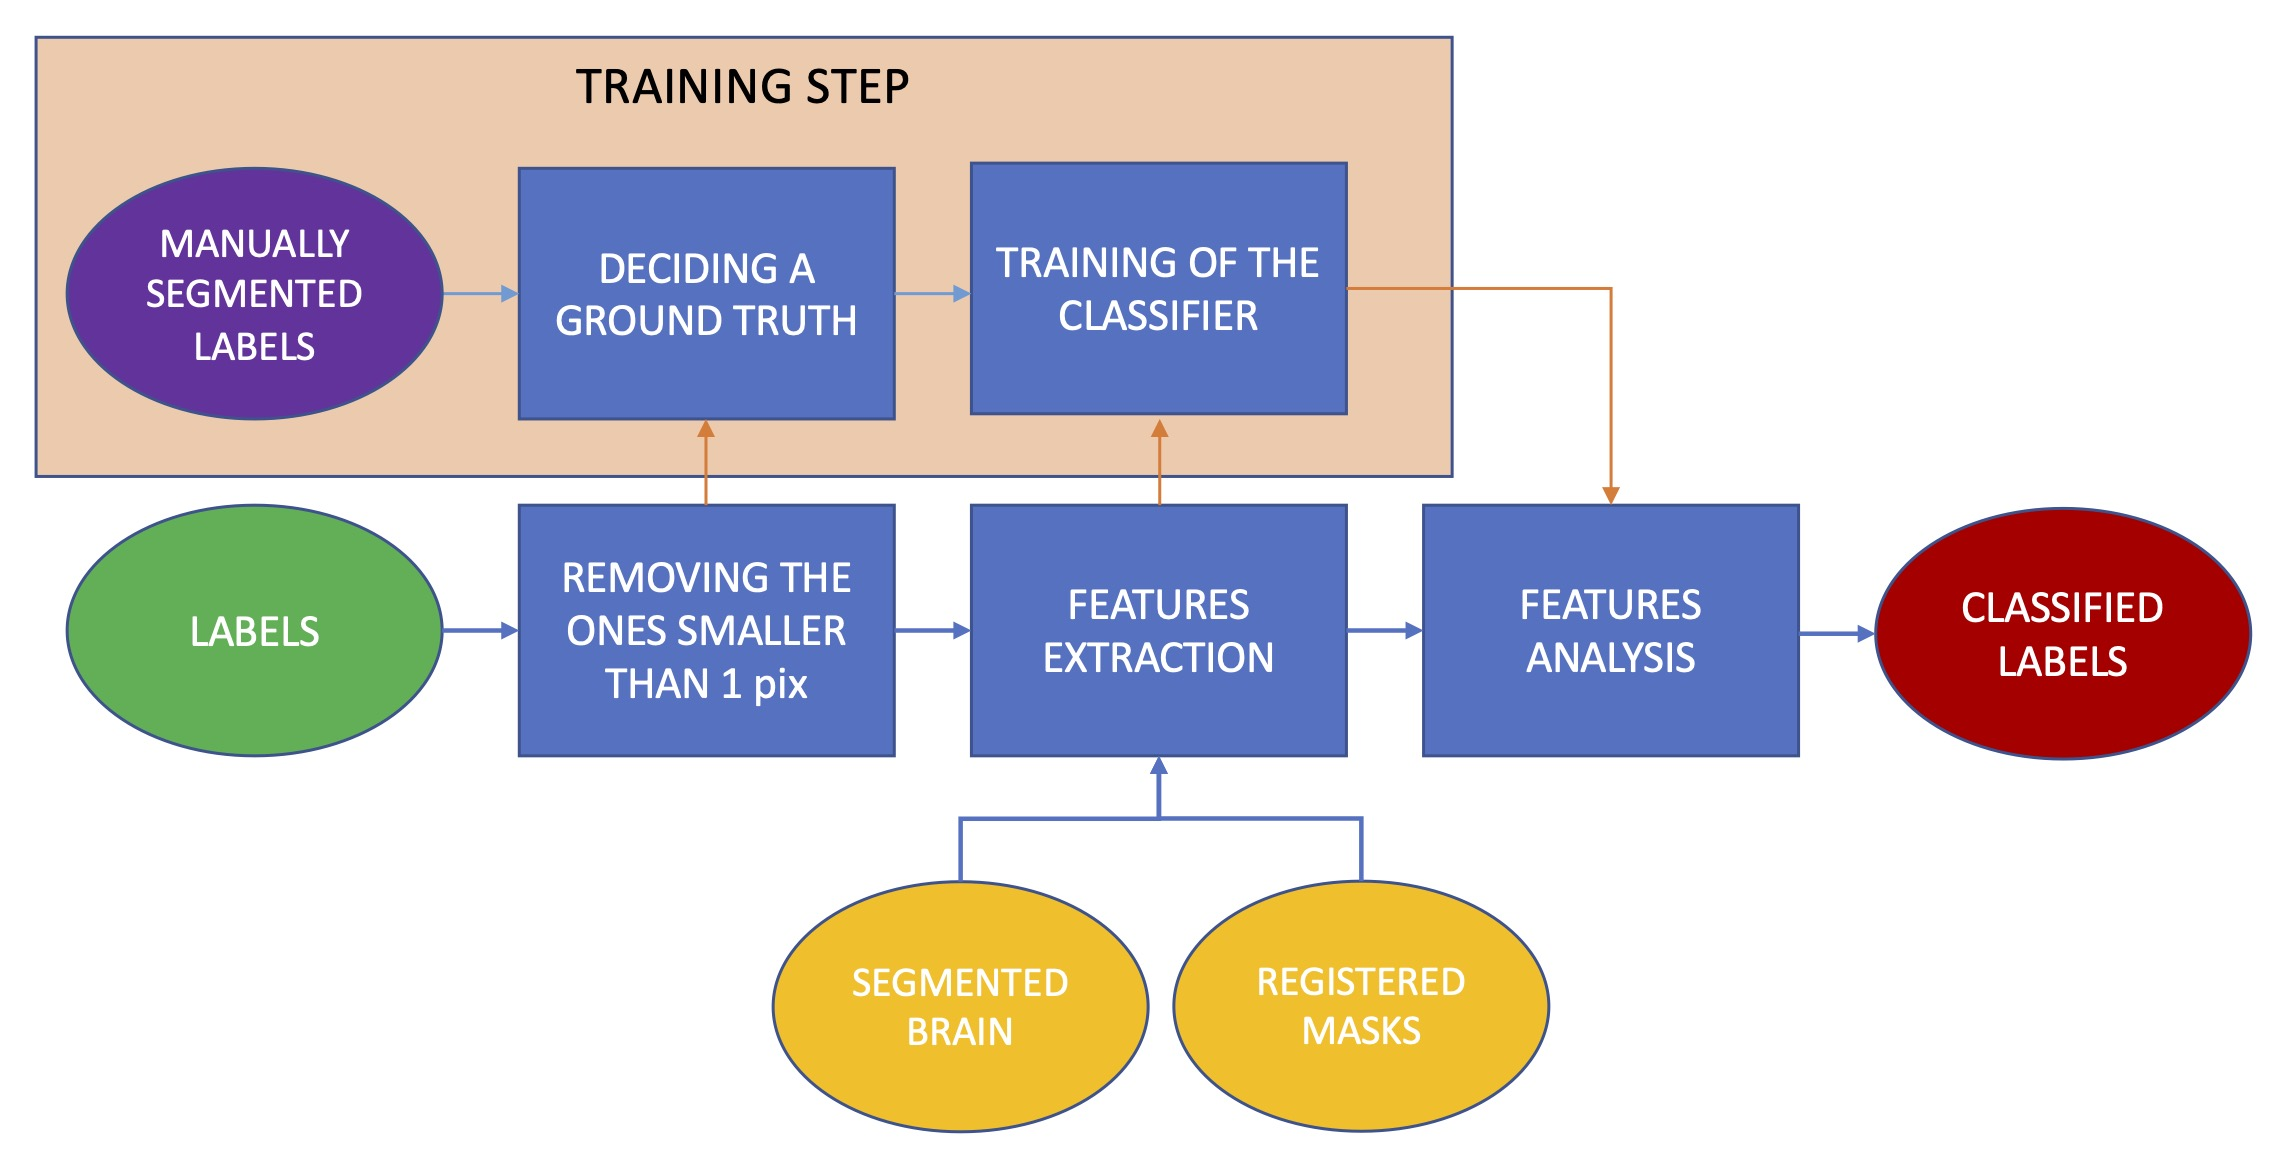
\includegraphics[scale = 0.16]{img/Chap2/FLOWCHART_POST.jpg}
    \caption{Workflow of the developed post-processing pipeline. In the flowchart is reported also the training of the classifiers which will be necessary only in the developing step. Once the classifiers are trained they can be used straightly on the new scans proposed.  }
    \label{fig:flowchart_post}
\end{figure}

\subsection{Description}

The post processing pipeline has to classify the labels obtained by the U-Net ensemble as true or false.

Traditionally, SCI must be greater that $3 mm$ in greatest linear dimension \cite{ART:Debaun} and visible in at least two planes \cite{Art:Casella}. 
Since the MRI has been improved and the 3D imaging became more often used this definition no longer holds strictly, but assure that, on the time this work of thesis was done, SCI's label can't be too small.
For those reason the first operation done on the results of the automatic segmentation was to remove all the labels smaller than two voxels. Even if the scans of the data set has an high variability in term of spacing, it was chosen to consider the number of voxels of the lesion instead of the physical space because the U-Net ensemble only consider single slices as 2D images.

The next step was the training of a classificator to decide if a segmented SCI has to be considered true based on features that will be discussed further on in this section.
Different classifiers was attempted to reach the best possible results, as it will showed in the next Chapter.
Both the training and the testing of the classifier was possible thanks to the provided manual segmentation of the SCIs, used as a ground truth.

\subsubsection{Ground Truth}
The first task to perform in order to obtain a good classifier was to decide how the automatically segmented lesions has to be considered true or false. That is needed since even the labels for the corrected segmented lesions often wasn't perfectly superimposable on the ground truth label.
This need was satisfied using a metric which is a modified version of the Jaccard index which is capable to take in account for the cases in which a single label obtained with the U-Net ensemble overlaps two or more labels of the manual segmentation.
The mathematically expression of the used index in reported in equation \ref{eq:modified_jaccard}.

\begin{equation} \label{eq:modified_jaccard}
    score(X) = \frac{|X \cap (Y_1 \cup Y_2 \cup ... \cup Y_n)|}
    {|X \cup (Y_1 \cup Y_2 \cup ... \cup Y_n)|}
\end{equation}
Where $X$ represents the set of pixel of the automatically segmented label, $Y_i$ represents one of the ground truth label that overlaps $X$ and $n$ is the number of the overlapped ground truth labels.
To consider the \textit{a priori} truth value of a single label obtained with the U-Net were manually compared the automatic segmentation of the SCIs with the ground truth and were chosen to keep a value of $0.25$ for the modified Jaccard index as a minimum threshold to consider the label true.

\subsubsection{Feature Extraction}

The next step was to choose which features to extract for the automatically segmented labels.
The features extracted where the followings:
\begin{itemize}
    \item The mean probability value of a label given by the U-Net;
    \item The total volume of the label measured in $mm^3$;
    \item The overlapping of a segmented label with a determined mask in which the probability of finding SCI is higher. The overlapping was measured computing the fraction of the pixels of the label that overlaps the selected mask over the total number of pixels of the label. It was again chosen to use the number of pixel because the U-Net ensemble only consider one slice per time;
    \item The overlapping of a segmented label with a determined mask in which the probability of finding SCI is lower. The overlaping was measured in the same way as for the previous point;
    \item The probability of a label to be in the white matter considering the partial volume map of the atlas. This probability was evaluated averaging the probability of each pixel of the label over the total number of pixels of the lesion;
    \item The probability of a label to be in the grey matter;
    \item The probability of a label to be in the cerebrospinal fluid;
\end{itemize}

The first feature comes from the output of the U-Net. The segmentation neural network returns a probability for each pixel to be part of a lesion. The mean value for the pixels of each label was taken.

The volume of a lesion was taken because, since the nature and the given definition of a SCI, the probability of finding very large or very small lesion is low.

Two binary masks were provided by expert clinicians from the University of Padua.
The first one is a mask of the boundary region of brain arteries and the cortical zone that in this work thesis will be called \textit{boundary region}. This is the region where the SCIs are more localized since the global reduction in arterial oxygen content and the cerebral hemodynamic factors seems to drive the ischemic mechanism \cite{ART:Ford}. An example of the applied mask can be seen in \figureautorefname~\ref{fig:boundary}
The second is a mask of the ventricular and periventricular regions in the brain. Those regions have a great probability to lead to false positive due to their structure which often lead to high intensity zone in a FLAIR scan for normal anatomical factors. This mask will be called \textit{exclusion region} and an example can be seen in \figureautorefname~\ref{fig:exclusion}.
Those mask were manually segmented on the MNI 152 atlas and then registered on each image analysed.
The overlapping between a label and a certain mask was calculated averaging the number of pixels in the mask over the total number of pixels in the label, as showed in the equation \ref{eq:probability_boundary_mask}.

\begin{equation}\label{eq:probability_boundary_mask}
    P(X \in Y) = \frac{|X \cap Y|}{|X|}
\end{equation}
Where X is the set of pixels of a label and Y is the set of pixels in the mask.

\begin{figure}[h!]
		\centering
        \begin{subfigure}[b]{0.49\textwidth}
        \centering
             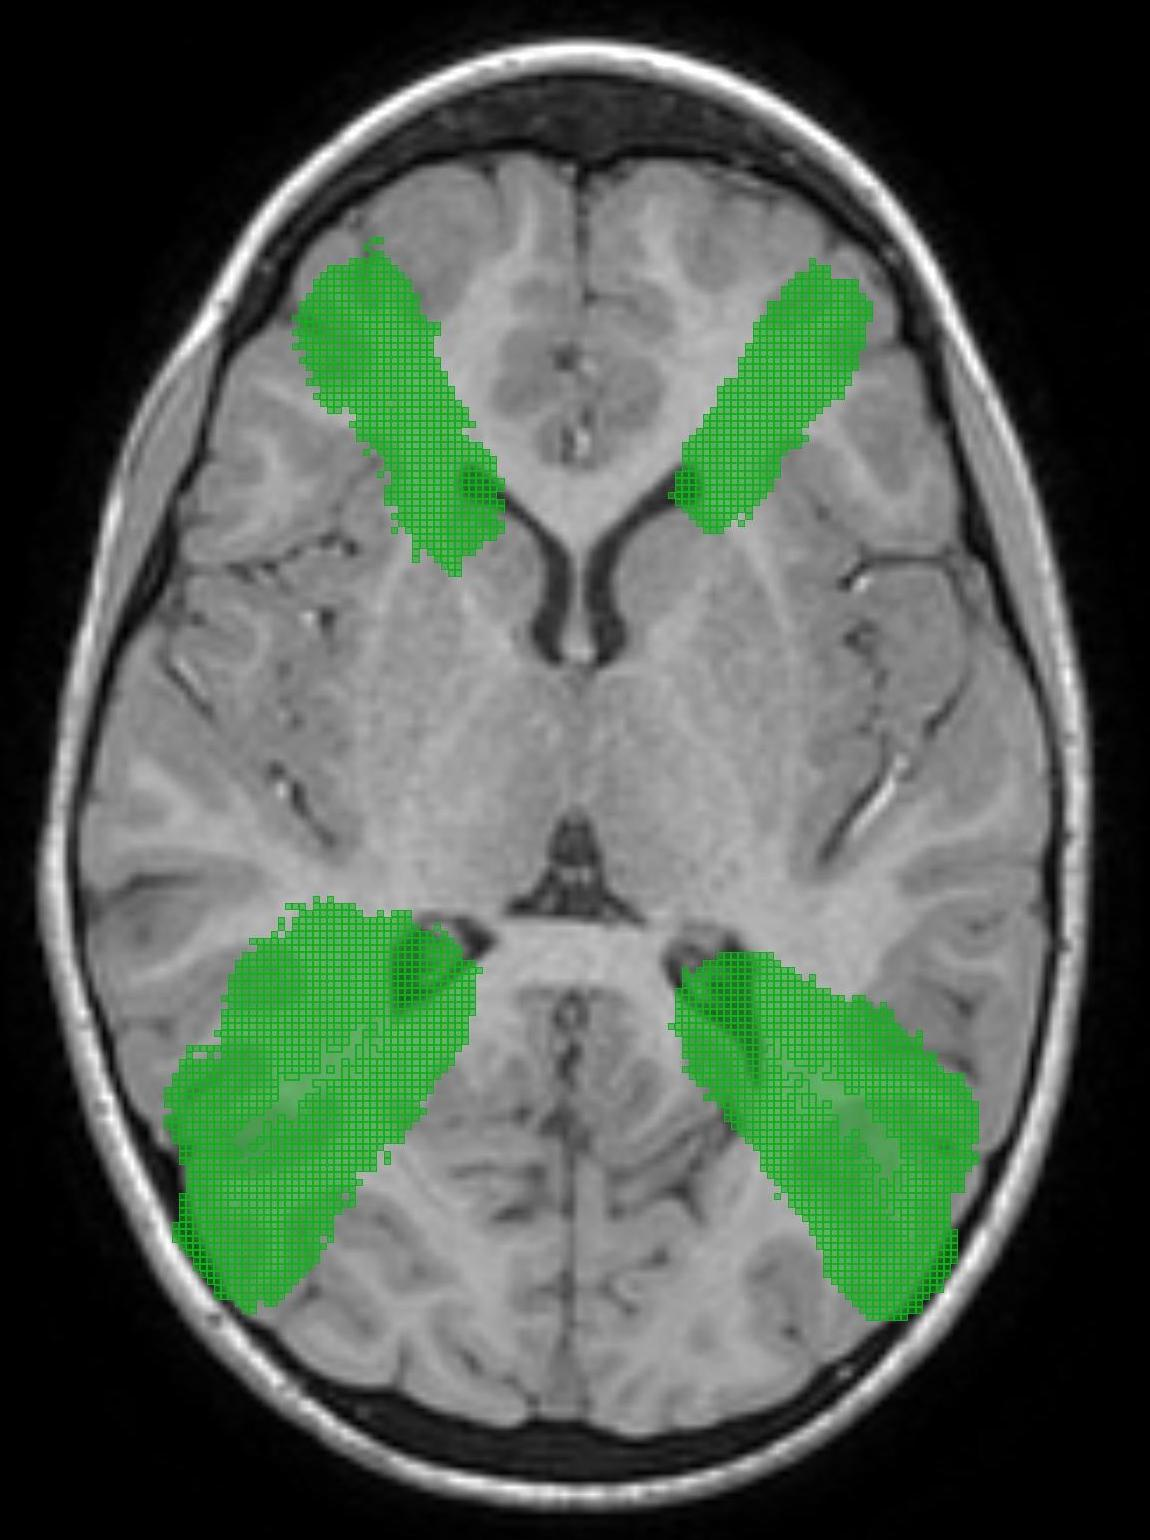
\includegraphics[scale=0.18]{img/Chap2/boundary.jpg}
             \caption{Boundary Zone} \label{fig:boundary}
        \end{subfigure}
        \hfill
        \begin{subfigure}[b]{0.49\textwidth}
        \centering
             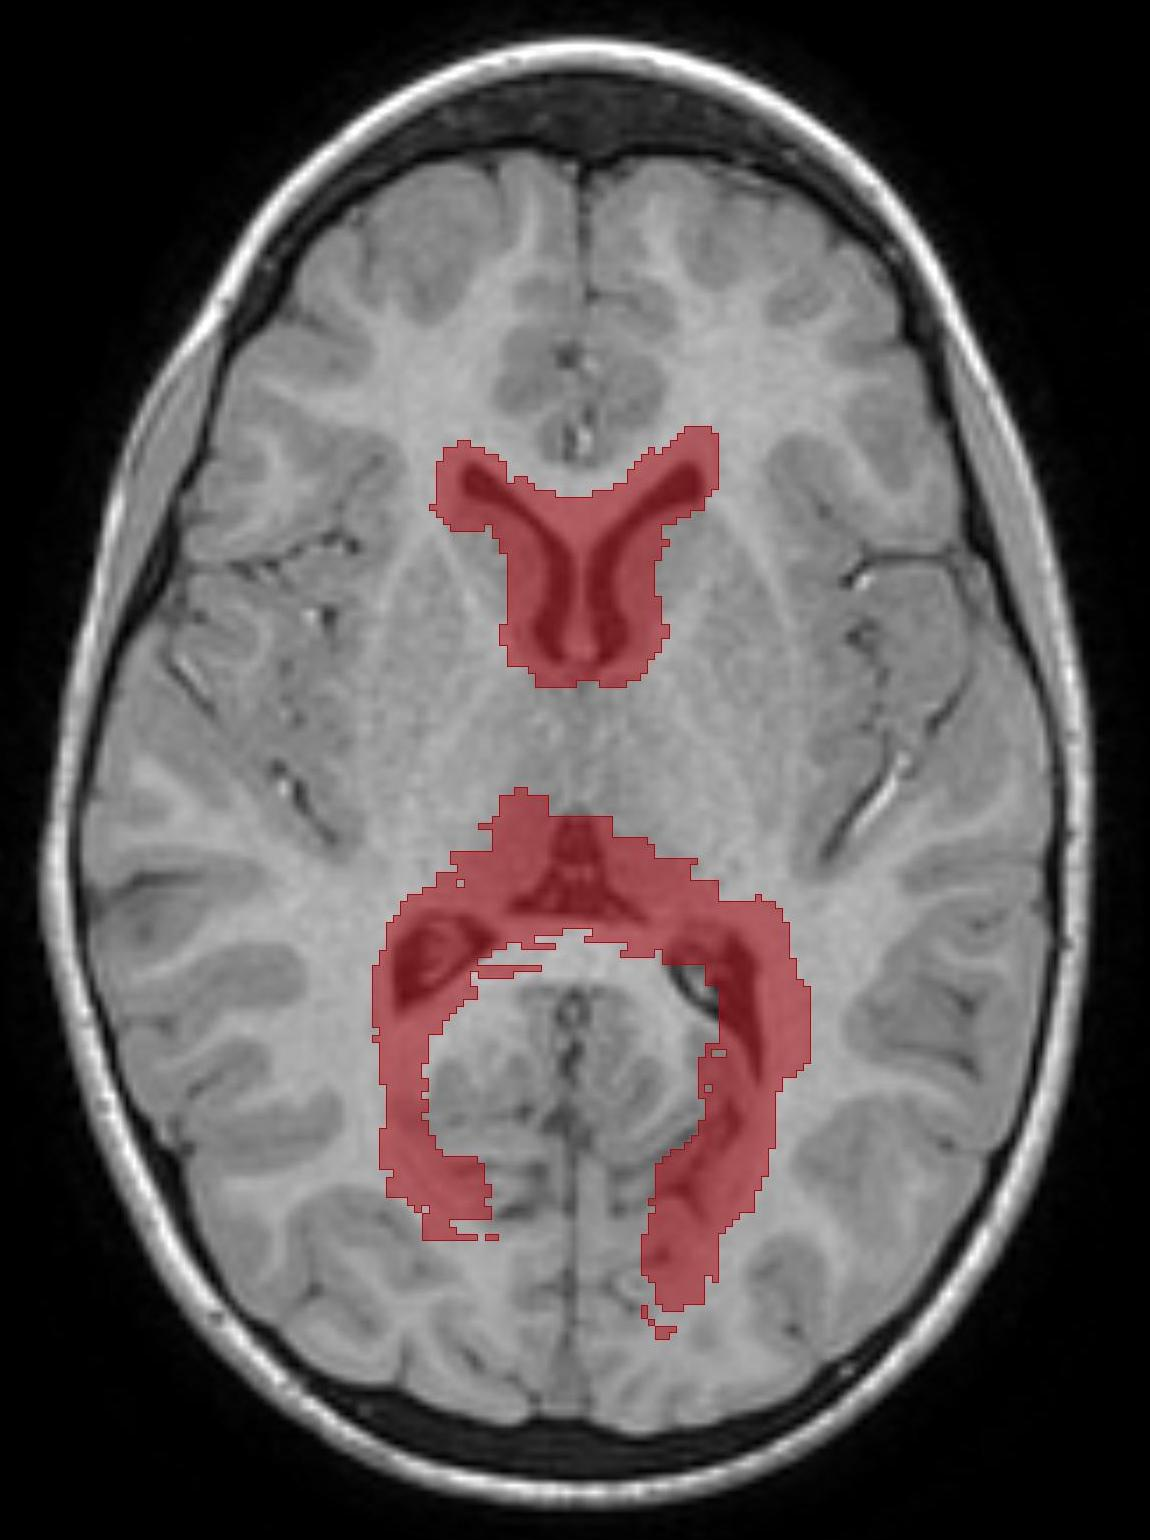
\includegraphics[scale=0.18]{img/Chap2/exclude.jpg}
             \caption{Exclusion Zone}\label{fig:exclusion}
        \end{subfigure}
        \caption{In Figure are reported an example of the masks used to evaluate the localization of a label registered over a patien volume. In Figure a is possible to see the region where the SCIs are usually more localized due to the anatomy of the human brain \cite{ART:Howing}, and in Figure b a zone which tends to naturally give hyperintense zones in the FLAIR image due to the walls of the ventricles. Both the masks were manually segmented by two expert clinicians of the University of Padua on the MNI152 atlas \cite{MNI152_09a} and then registered on each valued image.}\label{fig:masks}
\end{figure}


The probability of a label of being localized in a determined tissue therefore was obtained using the maps of the partial volume effect obtained in the pre-processing stage, having in this way a feature calculation which is based on the proper anatomy of each brain. This features were extracted in order to keeping in account both the medical evidence of the SCI to be more localized into the deep white matter \cite{ART:Howing}, and the working proper of the U-Net ensemble, which consider only one slice per time and therefore could suffer the partial volume effect.
For each tissue the probability of a label to belong to that tissue was calculated averaging the probability of each pixel over the total number of pixel in a label as the equation \ref{eq:probability_tissue_mask} shows.

\begin{equation}\label{eq:probability_tissue_mask}
    P(X \in A) = \frac{\sum_i P(x_i \in A)}{|X|}
\end{equation}
Where $A$ is the considered tissue (WM, GM or CSF), $X$ the set of pixels of a label and $x_i$ is a pixel of the label. The probability $P(x_i \in A)$ is given by the probability maps returned by the pre-processing segmentation.

\subsubsection{Training}
A set of two classifiers were then trained taking in input both a 2 dimensional array of features ($ Nsamples \times Nfeatures = Nsamples \times 7$) and a single dimensional array reporting the ground truth classification of each label, obtained starting from the manual segmentation and calculated as explained above.
The classifiers chosen were a \emph{Decision Tree} a \emph{Random Forest} and a \emph{Logistic Regression} classifiers.
The Decision Tree was chosen because of its interpretability and its capability to mimic the human decision process.
The Random Forest was attempt because of its higher resilience to overtraining and its usually highly performances with respect to decision tree.
The Logistic Regression was implemented due to the possibility of return a probability for each classification.

The complete data set was divided in two independent subsets, the first one, composed of $51$ patient's scans, was used during the training stage, the second one, composed of $6$ patients' scan was used for the test stage. In order to keep in account of all the possible variables the full data set was divided in order to obtain both the training and the test data set heterogeneous in terms of center or provenience, physical size of the automatically segmented labels and possible outcomes of the ground truth (i.e. possibility for a patient to be healthy and really not having SCI's evidences).

The training set was composed of the images of $51$ patients and totally counted $5581$ automatically obtained labels. This set was found to be highly unbalanced since approximately only the $3.7\%$ was labels classified as true.
To obtain a better training two resampling algorithms where used that permitted to obtain a better balancing for the two classes.

Firstly a \emph{SMOTE} \cite{ART:SMOTE} algorithm where used to add data to the less populated class. The SMOTE is a resampler algorithm that permits to artificially generate new data starting from the existing ones.
The more populated class was then undersampled with a random resampler algorithm, which randomly take out data from the selected class.

The parameters of the implemented classifiers were found using a \textit{Grid Search Cross Validation}, a process that permits to find the best parameters combination automatically maximizing a predetermined metric in a \textit{cross validation} test.
The cross validation process consists in the division of the given set (in this case the training set in to n subsets, $n-1$ of those subsets are used for training the classifier and the remaining one is used for test, measuring a predetermined metric, then the operation is repeated changing every time the test subset and finally averaging the obtained score.
The grid search operation consists in repeating the cross validation test for every possible parameters combination, permitting to find the one that obtain the maximum value for the chosen metric.
In this case also the parameters for the resamplers was found using the Grid Search, but generally for the SMOTE the output ratio between the minority and majority class ranged between $0.2$ and $0.3$ and for the random undersampler the output ratio found was between $0.6$ and $0.7$ for each classifier.

\subsection{Implementation}

The post processing pipeline was implemented using Python. To perform the essential operations the same libraries used on the pre-processing stage where used: \textsc{ITK} \cite{ART:ITK} and \textsc{Numpy} \cite{Numpy}.
To perform the classification the automatically segmented label two libraries were used: \textsc{Scikit-Learn} \cite{scikit-learn} and \textsc{Imbalanced-Learn} \cite{Imbalanced-Learn}.
The whole code is opensource and freely available on GitHub \cite{Neuroradiomics}.
During the developement, the installation was automatically tested on Ubuntu for
different python versions. This continuos integration process was carried out using
the github actions.

\subsubsection{Feature Extraction}

The first need was to distinguish and enumerate the labels for both the ground truth and the output labels uniquely.
This was obtained implementing a function that finds the connected regions on an image, which relies on an ITK filter already existing. The name of the function is self-explanatory.

Then the need was to quantify the agreement of automatically obtained label of the training set with the provided ground truth. This was obtained implementing a function that measure the modified Jaccard index as shown in equation\ref{eq:modified_jaccard} and then selecting only those lables that reaches a score higher than $0.25$.

\documentclass{standalone}




\begin{document}




\lstset{style=python}
	\begin{lstlisting}[language = python, caption = Modified Jaccard Index, label =modified_jaccard]
import itk
import numoy as np

def find_Jaccard_truth_value (counted_label, gnd_label, threshold = 0.25):
    
    #FINDING NUMBER OF LABELS
    maximum_filter = itk.MinimumMaximumImageCalculator[type(counted_label)].New()
    maximum_filter.SetImage(counted_label)
    maximum_filter.ComputeMaximum()
    num_labels = maximum_filter.GetMaximum()
    
    count_labels = np.array([0] * num_labels) #total number of pixels for lesion
    value_array = np.array( [False] * num_labels ) #array that reports what label is true
    
    #FINDING NUMBER OF GND TRUTH LABELS    
    counted_gnd = find_connected_regions(gnd_label)
    maximum_filter = itk.MinimumMaximumImageCalculator[type(counted_gnd)].New()
    maximum_filter.SetImage(counted_gnd)
    maximum_filter.ComputeMaximum()
    num_gnd = maximum_filter.GetMaximum()
    
    count_gnd = np.array( [0] * num_gnd ) #total number of pixels for lesion
    
    overlapping_matrix = np.array( [[0]*num_gnd]*num_labels)
    jaccard_index = np.array([0.]*num_labels)
    index = itk.Index[3]()

    for index[0] in range( counted_label.GetLargestPossibleRegion().GetSize()[0] ):
            for index[1] in range( counted_label.GetLargestPossibleRegion().GetSize()[1] ):
                for index[2] in range( counted_label.GetLargestPossibleRegion().GetSize()[2] ):
                    if counted_gnd.GetPixel(index) != 0 :
                        count_gnd[ counted_gnd.GetPixel(index)-1] +=1
                    if counted_label.GetPixel(index) != 0 :
                        count_labels[ counted_label.GetPixel(index)-1] +=1
                        if counted_gnd.GetPixel(index) != 0 :
                            overlapping_matrix[counted_label.GetPixel(index) - 1][counted_gnd.GetPixel(index)-1] += 1
                            
    num = np.array([0]*num_labels)
    den = np.array([0]*num_labels)
    
    for i in range(num_labels):
        for j in range(num_gnd):
            num[i] += overlapping_matrix[i][j]
            if overlapping_matrix[i][j]!= 0 : den[i] += count_gnd[j]
        den[i] += count_labels[i] - num[i]
        
        jaccard_index[i] = num[i]/den[i]
        
        value_array[i] = (jaccard_index[i] >= threshold)
        
    return value_array, jaccard_index


\end{lstlisting}


\end{document}

Once the labels of the training set have been classified as true or false the subsequent step was to properly extract the cited features.

The features extracted was the mean of the probability values given by the U-Net for the pixels in a label; the volume of the label, obtained multiplying the number of the voxels in a label for the voxel dimension; the mean of overlapping with two binary masks (boundary region and exclusion region) and the mean value for the overlapping with three probability masks (WM, GM, CSF).
Since the boundary and exclusion region are binary the overlapping has been taken in the same way the mean probability of belonging to a determined tissue was calculated. This permitted to implement a function that take as input only two parameters: the image with the labels and a list of masks.

The feature extracted therefore had different magnitude and also there was the possibility that some features was an outlier. Outliers are defined as an observation which deviates a lot from other observations to arouse suspicion that was generated by a different mechanism in a data set \cite{ART:outliers}.
To have a better distribution of the data the obtained features was then applied a scaler, i.e. an algorithm capable to normalize the data in order to have all the same order of magnitude.
The applied algorithm was the function \emph{Robust Scaler} from the library Scikit-Learn \cite{scikit-learn}, which computes the median and the interquartile range (IQR) for each feature of the data set proposed and then remove the medians for each feature and scales them according to the IQR \cite{RobustScaler}.
Usually features scaling the mean and the variance are used, but those metrics tend to be badly affected by the outliers, this approach is more robust toward outliers and permits better results.

\documentclass{standalone}

\begin{document}




\lstset{style=python}
	\begin{lstlisting}[language=python, caption = Feature Extracion, label=feature_extraction]
import itk
import numpy as np
from sklearn.preprocessing import RobustScaler

def feature_scoring (label_img, masks_list):
    #binarize the labels
    bin_label = binarize (label_img, 0.5)
    
    #differentiating the labels
    counted_label = find_connected_regions (bin_label)
    #Calculating the volume of a voxel
    voxel_volume = label_img.GetSpacing()[0] * label_img.GetSpacing()[1] * label_img.GetSpacing()[2] 
    
    #FINDING NUMBER OF LABELS
    maximum_filter = itk.MinimumMaximumImageCalculator[type(counted_label)].New()
    maximum_filter.SetImage(counted_label)
    maximum_filter.ComputeMaximum()

    index = itk.Index[3]()
    pounded_score = np.array( [[0.] * (len(masks_list) + 2)] * maximum_filter.GetMaximum() ) #score for lesions divided pixels per lesion
    score = np.array( [[0.] * (len(masks_list) + 2)] * maximum_filter.GetMaximum() ) #total scores for each lesion
    count = np.array( [0.] * maximum_filter.GetMaximum() ) #total number of pixels for lesion
    
    for index[0] in range( label_img.GetLargestPossibleRegion().GetSize()[0] ):
        for index[1] in range( label_img.GetLargestPossibleRegion().GetSize()[1] ):
            for index[2] in range( label_img.GetLargestPossibleRegion().GetSize()[2] ):
                if label_img.GetPixel(index) != 0 :
                    count[counted_label.GetPixel(index) - 1] += 1
                    score[counted_label.GetPixel(index) - 1][0] += label_img.GetPixel(index)
                    for i in range(len(masks_list)):
                        score[counted_label.GetPixel(index) - 1][i + 2] += masks_list[i].GetPixel(index)
              
    for i in range(len(score)):
        pounded_score[i][0] = score[i][0] / count[i]
        pounded_score[i][1] = voxel_volume * count[i]
        
        #everything in the mask must be averaged
        for j in range( 2, len(score[i]) ):
            pounded_score[i][j] = score[i][j] / count[i]
    
    return pounded_score, counted_label
    
def robust_scaling(data, transformer = None):

    if transformer == None:
        transformer = RobustScaler().fit(data)
        
        new_data = transformer.transform(data)
    return new_data, transformer
    \end{lstlisting}


\end{document}

\subsubsection{Training}

Once the features were extracted for the labels of the training set, then it was possible to define and train the classifiers.
For both classifiers the parameter \textit{class\_weight} was set as \textit{'balanced'} since, in this way, the fitting algorithm would have taken in account the unbalancing of the training set.
All the other parameters were automatically chosen using a \emph{grid search} algorithm.
The metric that where chose to maximize was the AUC precision-recall score, which keeps in account both the precision and recall and is usually a valid choice to estimate goodness of unbalanced data classification.


\documentclass{standalone}




\begin{document}




\lstset{style=python}
	\begin{lstlisting}[language=python, caption=Training, label=training]
from sklearn.tree import DecisionTreeClassifier
from sklearn.linear_model import LogisticRegression
from imblearn.ensemble import BalancedRandomForestClassifier
from imblearn.over_sampling import SMOTE
from imblearn.under_sampling import RandomUnderSampler

dtc = Pipeline([
    ('SMOTE', SMOTE(sampling_strategy = 0.2, random_state = 42)),
    ('UnderSampler', RandomUnderSampler(sampling_strategy = 0.7, random_state = 42)),
    ('classification', DecisionTreeClassifier(random_state = 42, max_depth = 6, class_weight = 'balanced', criterion = 'entropy')) ])
dtc.fit(train_score, train_truth)

lr = Pipeline([
    ('SMOTE', SMOTE(sampling_strategy = 0.3, random_state = 42)),
    ('UnderSampler', RandomUnderSampler(sampling_strategy = 0.7, random_state = 42)),
    ('classification', LogisticRegression(random_state = 42, class_weight = 'balanced', penalty = None, solver = 'lbfgs', max_iter = 10000)) ])
lr.fit(train_score, train_truth)

brfc = Pipeline([
    ('SMOTE', SMOTE(sampling_strategy = 0.2, random_state = 42)),
    ('UnderSampler', RandomUnderSampler(sampling_strategy = 0.6, random_state = 42)),
    ('classification', BalancedRandomForestClassifier(
        random_state = 42, 
        class_weight = 'balanced',
        criterion = 'entropy', 
        max_depth = 8, 
        max_features = None,
        n_estimators = 1000,
        n_jobs = 10)) ])
brfc.fit(train_score, train_truth)
\end{lstlisting}


\end{document}



\end{document}